
% Slideshow, written by Brent Baccala, for a lecture at TJHSST

\documentclass{beamer}
\usetheme{Madrid}

\title{A New Solution to Hydrogen}
\author{Brent Baccala}
\institute{\tt cosine@freesoft.org}
%% \date{February 8, 2023}

\setbeamertemplate{footline}{}
\beamertemplatenavigationsymbolsempty

\usepackage{amsmath}
\usepackage{tabularx}

\usepackage{breqn}

\usepackage{xcolor}
\usepackage{comment}
\usepackage{graphicx}

\usepackage{tabularx}

\usepackage{listings}

\usepackage{fancyvrb}

\usepackage{soul}

\usepackage{tikz}
\usetikzlibrary{positioning}
\usetikzlibrary{fit}
\usetikzlibrary{calc,arrows.meta}
\usetikzlibrary{backgrounds}
\usetikzlibrary{angles,quotes,3d}
\usepackage{tikz-3dplot}

\usepackage{pgfplots}

\pgfmathdeclarefunction{gauss}{2}{%
  \pgfmathparse{1/(#2*sqrt(2*pi))*exp(-((x-#1)^2)/(2*#2^2))}%
}

\usepackage{adjustbox}

\def\coeff{\framebox(10,10){}}
\newcommand{\tikzmark}[1]{\tikz[overlay,remember picture] \node (#1) {};}

\begin{document}


\begin{frame}
\titlepage
\begin{block}{Abstract}
\begin{itemize}
\item An Introduction to Wave Mechanics
\item The Classical Solutions to the Hydrogen Schr\"odinger Equation
\item A New Solution to the Hydrogen Schr\"odinger Equation
\item Further Research Directions: Helium's Ground State
\end{itemize}
\end{block}
\end{frame}

\begin{frame}
\begin{exampleblock}{}
\begin{center}
\vskip 20pt
\Huge
Part 1: Schr\"odinger's Equation
\vskip 6pt
\ 
\end{center}
\end{exampleblock}
\end{frame}

\begin{frame}
\frametitle{Force, Field, Potential, Potential Energy}
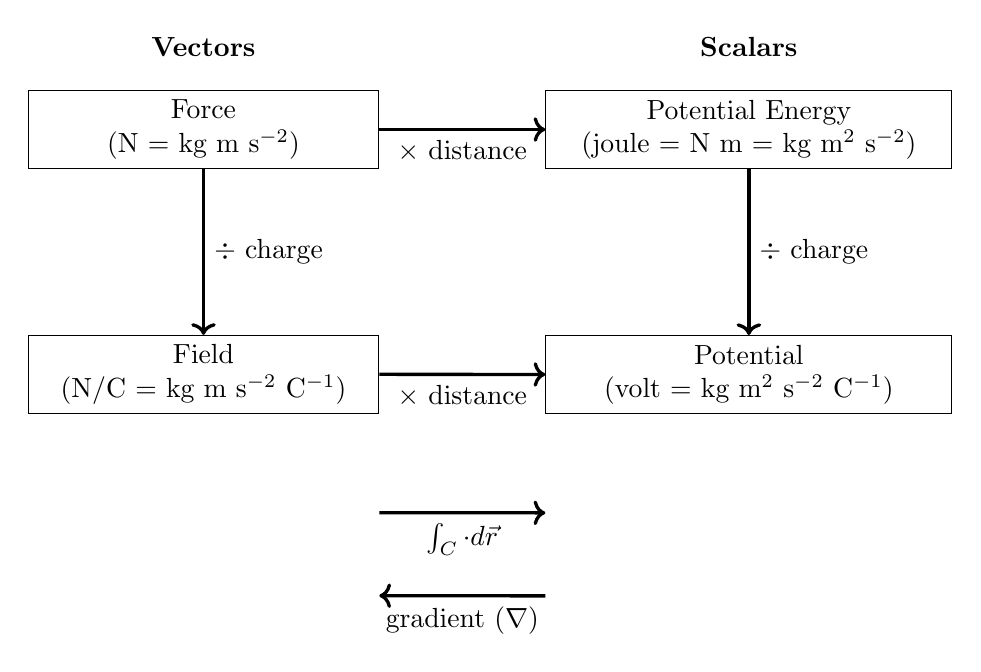
\begin{tikzpicture}[node distance=60pt]
\node (force) [draw, text width=120pt, align=center] {Force\\(N = kg m s$^{-2}$)};

\node (field) [below=of force.south, draw, text width=120pt, align=center] {Field\\(N/C = kg m s$^{-2}$ C$^{-1}$)};

\node (energy) [right=of force.east, draw, text width=140pt, align=center] {Potential Energy\\(joule = N m = kg m$^2$ s$^{-2}$)};

\node (potential) [below=of energy.south, draw, text width=140pt, align=center] {Potential\\(volt = kg m$^2$ s$^{-2}$ C$^{-1}$)};

\draw [very thick, ->] (force.south) -- (field.north) node[pos=0.5,right] {$\div$ charge};
\draw [very thick, ->] (energy.south) -- (potential.north) node[pos=0.5,right] {$\div$ charge};
\draw [very thick, ->] (force.east) -- (energy.west) node [pos=0.5, below] {$\times$ distance};
\draw [very thick, ->] (field.east) -- (potential.west) node [pos=0.5, below] {$\times$ distance};

\draw [very thick, ->] ([yshift=-50]field.east) -- ([yshift=-50]potential.west) node [pos=0.5, below] {$\int_C \cdot d\vec{r}$};
\draw [very thick, <-] ([yshift=-80]field.east) -- ([yshift=-80]potential.west) node [pos=0.5, below] {gradient ($\nabla$)};

\node [above of=force, node distance=30pt] {\bf Vectors};
\node [above of=energy, node distance=30pt] {\bf Scalars};
\end{tikzpicture}
\end{frame}

\begin{comment}

\begin{frame}
\frametitle{Lagrangian Mechanics}
\begin{definition}[the Lagrangian]
\[ L = T - V \]
%\[ S = \int_{t_1}^{t_2} L(x, \dot x, t) dt \]
\begin{center}
T is kinetic energy \qquad\qquad V is potential energy
\end{center}
\end{definition}

\begin{block}{The Euler-Langrange (E-L) equation}
\[ \frac{d}{dt}\left( \frac{\delta L}{\delta \dot x} \right) = \frac{\delta L}{\delta x} \]
\end{block}

\begin{center}

In one dimension:

\[ L = \frac{1}{2} m \dot x^2 - V(x) \]

\[ \frac{d}{dt}\left( m \dot x \right) = - \frac{d V}{d x} = F\]

\end{center}

\end{frame}

\begin{frame}
\frametitle{Lagrangian Mechanics}
\begin{definition}[the action]
\[ S = \int_{t_1}^{t_2} L(x, \dot x, t) dt \]
\end{definition}

\[ L = T - V \]

\[ \frac{d}{dt}\left( \frac{\delta L}{\delta \dot x} \right) = \frac{\delta L}{\delta x} \]

\[ L = \frac{1}{2} m \dot x^2 = - \frac{dV}{dx} \]

\end{frame}

\begin{frame}
\frametitle{Hamiltonian Mechanics}

\begin{block}{Hamilton's equations}
\[ \dot q = \frac{\delta H(q,p)}{\delta p} \qquad\qquad \dot p = - \frac{\delta H(q,p)}{\delta q} \]
\end{block}

\end{frame}

\end{comment}

\begin{frame}
\frametitle{Classical Mechanics}

\begin{center}
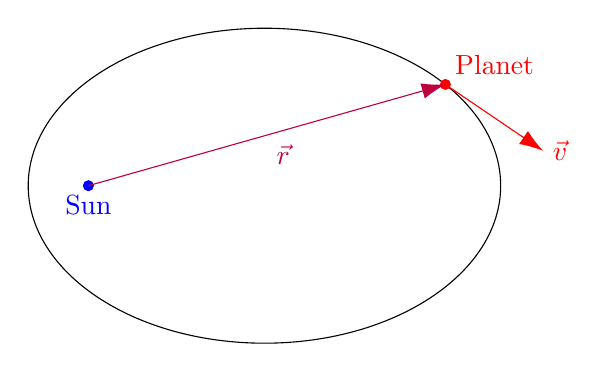
\begin{tikzpicture}
    % Define the parameters of the ellipse
    \pgfmathsetmacro{\majorAxis}{3}
    \pgfmathsetmacro{\minorAxis}{2}
    \pgfmathsetmacro{\angle}{40}
    \pgfmathsetmacro{\focusShift}{sqrt(\majorAxis^2 - \minorAxis^2)}

    % Draw the ellipse
    \draw (0,0) ellipse (\majorAxis cm and \minorAxis cm);

    % Define the point on the ellipse
    \coordinate (P) at (\angle:\majorAxis cm and \minorAxis cm);

    % Define the focus of the ellipse
    \coordinate (F) at (-\focusShift, 0);

    % Draw the points
    \fill[red] (P) circle (2pt) node[above right] {Planet};
    \fill[blue] (F) circle (2pt) node[below] {Sun};

    % Define a style for the large arrow
    \tikzset{large arrow/.style={-{Latex[length=3mm, width=2mm]}}}

    % Draw the tangent vector at point P
    \draw[large arrow, red] (P) -- ($(P)!1.5cm!90+\angle:(F)$) node [right] {$\vec{v}$};

    % Draw the vector from F to P
    \draw[large arrow, purple] (F) -- (P) node [midway, below right] {$\vec{r}$};
\end{tikzpicture}

\end{center}

Specify:
\begin{itemize}
\item Initial Position
\item Initial Velocity
\item One of: Force, Field, Potential, Potential Energy
\end{itemize}

\[ F = ma \qquad\qquad \frac{G m_1 m_2}{r^2} = m_1 a \]

\end{frame}

\begin{frame}
\frametitle{Probability Density Functions}

\begin{center}
In quantum mechanics, we can't compute the exact location of a particle;
we can only compute its {\it probability density function}.

\vskip 12pt

\begin{tikzpicture}
\begin{axis}[
  no markers,
  domain=0:10,
  samples=100,
  ymin=0,
  axis lines*=middle,
  xlabel=$x$,
  height=5cm,
  width=12cm,
  xtick={-1,1},
  xticklabels={$a$,$b$},
  ytick=\empty,
  enlargelimits=false,
  clip=false,
  axis on top,
  grid = major,
  grid style={dashed, gray!30},
]

\addplot [fill=cyan!20, draw=none, domain=-1:1] {gauss(0,1)} \closedcycle;

\addplot [very thick,cyan!50!black, domain=-5:5] {gauss(0,1)};

%% \draw [yshift=-0.6cm, latex-latex](axis cs:4,0) -- node [fill=white] {$1\sigma$} (axis cs:6,0);

\end{axis}
\end{tikzpicture}

The shaded area is the probability that the particle's measured x-coordinate will be between $a$ and $b$,
assuming that the total area under the curve is 1.
\end{center}

\end{frame}

\def\argt{(\vec{x}_1,...,\vec{x}_n,t)}
\def\arg{(\vec{x}_1,...,\vec{x}_n)}

\begin{frame}
\frametitle{The Wave Function}
\[ \Psi\argt \]

The {\bf wave function} is a complex-valued function of position and time that encodes
probability density functions for both the position and momentum of all particles.
It is a function of the coordinates of {\it all} particles.

\vskip 12pt
\begin{quotation}
Example: The wavefunction of a two particle system:

\[ \Psi(x_1,y_1,z_1,x_2,y_2,z_2,t) \]
\end{quotation}

The square amplitude of the wave function gives the probability density of the position.

The square amplitude of its Fourier transform gives the probability density of the momentum.

\[ \Phi(p) = \frac{1}{\sqrt{2\pi\hbar}}\int \Psi(x)e^{-\frac{i}{\hbar}px}dx \]
\end{frame}

\begin{frame}
\frametitle{(Time Dependent) Schr\"odinger Equation}
%% 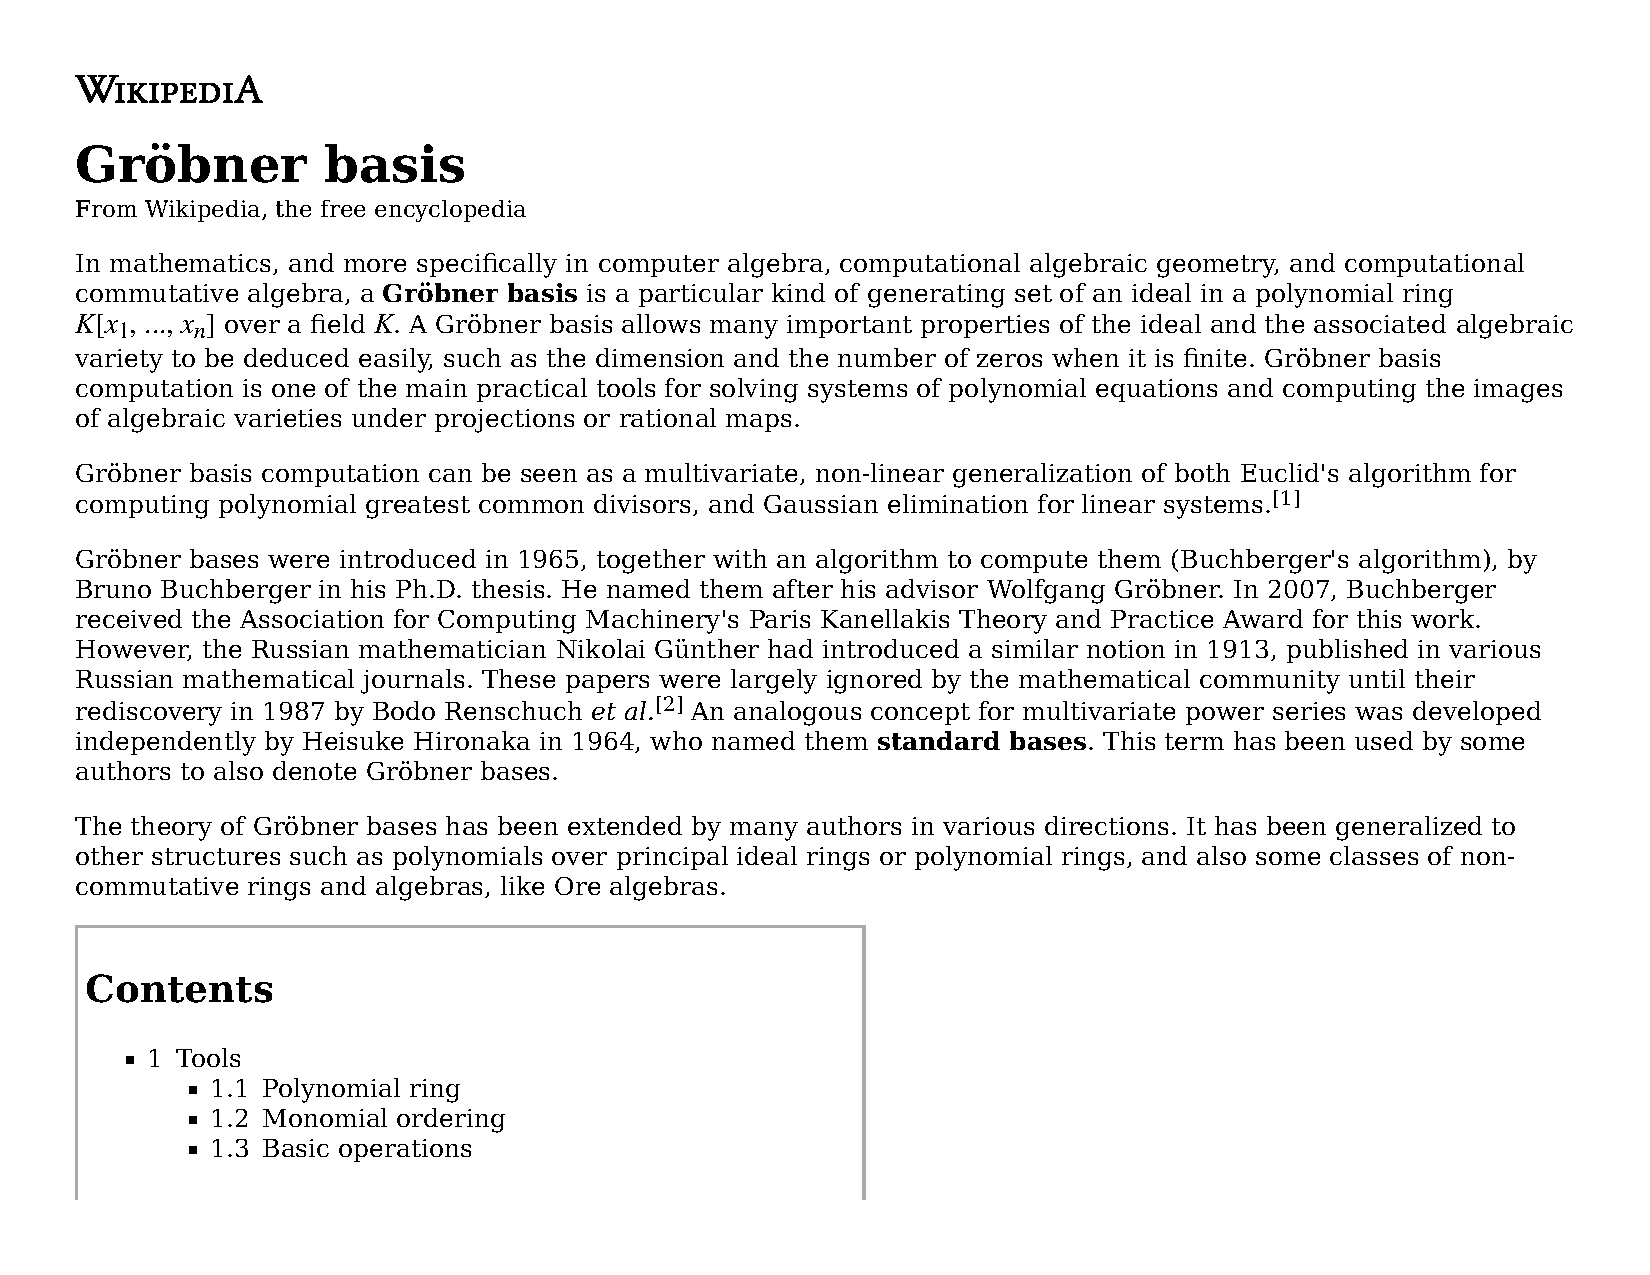
\includegraphics[clip, trim=0in 5.6in 0in 0.75in, width=\textwidth, page=1]{GrobnerBasis.pdf}
%% \includegraphics[clip, trim=0in 6.25in 0in 0.5in, width=\textwidth, page=9]{GrobnerBasis.pdf}
%% \includegraphics[clip, trim=0in 3in 0in 0.5in, width=\textwidth, page=13]{GrobnerBasis.pdf}
\begin{block}{}
\[ \hat{H} \Psi\argt = i \hbar \frac{\delta}{\delta t} \Psi\argt \]
\end{block}
%\vskip 0.3in
\begin{center}
\underline{{\bf Definition of Hamiltonian operator $\hat{H}$}}
\[ \hat{H} \Psi\argt = \hat{T} \Psi\argt + \hat{V} \Psi\argt \]

$\hat{T}$ is the kinetic energy operator \qquad
$\hat{V}$ is the potential energy operator

\vskip 12pt

Construct $\hat{T}$ and $\hat{V}$ like this:

\[\hat{T} = \sum_i - \frac{\hbar^2}{2m_i}\nabla_i^2 \qquad\qquad \hat{V} = V\argt\]

$\nabla_i^2$ is the {\it Laplacian} with respect to the $i\hspace{0.05em}^{\rm th}$ particle.
%% \[ \nabla_i^2 = \frac{\delta^2}{\delta x_i^2} + \frac{\delta^2}{\delta y_i^2} + \frac{\delta^2}{\delta z_i^2} \quad {\rm (cartesian\ coordinates)}\]

\vskip 12pt

The sum in $\hat{T}$ is over all particles.

\end{center}

\end{frame}

\begin{frame}
\frametitle{Vector Derivatives}

In two and three dimensional space, we often prefer to use coordinate-free notation for derivatives:

\vskip 12pt

The {\it gradient} $\nabla f$ of a scalar-valued function is a vector-valued function that gives the direction and rate of greatest increase.

\vskip 12pt

The {\it divergence} $\nabla \cdot \vec{F}$ of a vector-valued function is a scalar-valued function that gives the strength of a source.

\vskip 12pt

The {\it curl} $\nabla \times \vec{F}$ of a vector-valued function is a (pseudo)vector-valued function that gives the rotational strength of the vector field at each point.

\vskip 12pt

The {\it Laplacian} $\nabla^2 f$ or $\Delta f$ of a scalar-valued function is a second derivative, the divergence of the gradient.

\end{frame}

\begin{frame}
\frametitle{Vector Derivatives}

\[
\begin{array}{ccc}
 {\bf Operation}      & {\bf Cartesian\ coordinates}  & {\bf Spherical\ coordinates} \\
& & \\
 {\rm Vector\ field}\\ \vec{A} & A_x \vec{x} + A_y \vec{y} + A_z \vec{z} & A_r \vec{r} + A_\theta \vec{\theta} + A_\phi \vec{\phi} \\
& & \\
 {\rm Gradient} \\ \nabla f & \frac{\delta f}{\delta x}\vec{x} + \frac{\delta f}{\delta y}\vec{y} + \frac{\delta f}{\delta z}\vec{z} & \frac{\delta f}{\delta r}\vec{r} + \frac{1}{r} \frac{\delta f}{\delta \theta}\vec{\theta} + \frac{1}{r \sin\theta}\frac{\delta f}{\delta \phi}\vec{\phi} \\

& & \\
 {\rm Divergence}  & \frac{\delta A_x}{\delta x} + \frac{\delta A_y}{\delta y} + \frac{\delta A_z}{\delta z} & \frac{1}{r^2} \frac{\delta (r^2 A_r)}{\delta r} + \frac{1}{r \sin \theta} \frac{\delta}{\delta \theta}\left(A_\theta \sin\theta\right)\\
\nabla \cdot \vec{A}  & & + \frac{1}{r \sin\theta}\frac{\delta A_\phi}{\delta \phi} \\

& & \\
 {\rm Laplacian} & \frac{\delta^2 f}{\delta x^2} + \frac{\delta^2 f}{\delta y^2} + \frac{\delta^2 f}{\delta z^2} &   \frac{1}{r^2} \frac{\delta}{\delta r}\left(r^2\frac{\delta f}{\delta r}\right) + \frac{1}{r^2\sin\theta} \frac{\delta}{\delta \theta}\left(\sin\theta\frac{\delta f}{\delta\theta}\right) \\
\nabla^2 f  & & + \frac{1}{r^2 \sin^2\theta}\frac{\delta^2 f}{\delta \phi^2} \\

\end{array}
\]

Source: Wikipedia, {\it Del in cylindrical and spherical coordinates}

\end{frame}

\begin{comment}

\begin{frame}
\frametitle{Aside: Tensor Derivatives}

In higher dimensional spaces, vector derivative concepts fail and we prefer to use tensor calculus, the {\it exterior derivative},
the {\it musical isomorphisms} and the {\it Hodge star operator}.

\vskip 12pt

An {\it $n$-form} is (roughly) a $n$-dimensional differential.

The {\it exterior derivative} maps an $n$-form to an $(n+1)$-form.

The {\it musical isomorphisms} map back and forth between the tangent space and the cotangent space.

The {\it Hodge star operator} maps an $n$-form to an $(r-n)$-form, in $r$-dimensional space.

\[
\begin{array}{rcccl}
  \operatorname{grad} f &\equiv& \nabla f        &=& \left( d f \right)^\sharp \\
  \operatorname{div} F  &\equiv& \nabla \cdot F  &=& {\star d {\star} \mathord{\left( F^\flat \right)}} \\
  \operatorname{curl} F &\equiv& \nabla \times F &=& \left( {\star} d \mathord{\left( F^\flat \right)} \right)^\sharp \\
  \Delta f              &\equiv& \nabla^2 f      &=& {\star} d {\star} d f \\
                        &      & \nabla^2 F      &=& \left(d{\star}d{\star}\mathord{\left(F^{\flat}\right)} - {\star}d{\star}d\mathord{\left(F^{\flat}\right)}\right)^{\sharp} \\
\end{array}
\]

Source: Wikipedia, {\it Exterior derivative}

\end{frame}

\end{comment}

\begin{frame}
\frametitle{Time Independent Schr\"odinger Equation}
If the potential energy $V\argt$ has no time dependence, we can 
use separation of variables and {\it assume} that the wavefunction has the form:

\[ \Psi\argt = \psi\arg\phi(t) \]

\[\sum_i - \frac{\hbar^2}{2m_i}\nabla_i^2 \psi\arg\phi(t) + V\arg\psi\arg\phi(t) \]
\[ = i \hbar\frac{\delta}{\delta t} \psi\arg\phi(t) \]

divide through by $\psi\arg\phi(t)$:

\[ \frac{1}{\psi\arg} \left[ \sum_i - \frac{\hbar^2}{2m_i}\nabla_i^2 \psi\arg + V\arg\psi\arg \right] \]
\[ = \frac{i\hbar}{\phi(t)} \frac{\delta}{\delta t} \phi(t) \]

\end{frame}

\begin{frame}
\frametitle{Time Independent Schr\"odinger Equation}
The time part:

\[ E = \frac{i\hbar}{\phi(t)} \frac{\delta}{\delta t} \phi(t) \quad\Rightarrow\quad - \frac{i E \delta t}{\hbar} = \frac{\delta\phi(t)}{\phi(t)} \quad\Rightarrow\quad - \frac{i E t}{\hbar} + C = \ln \phi(t) \]
\[ \phi(t) = e^C e^{-iEt/\hbar}\]

The position part:

\[ \frac{1}{\psi\arg} \left[ \sum_i - \frac{\hbar^2}{2m_i}\nabla_i^2 \psi\arg + V\arg\psi\arg \right] = E \]

\[ \left[ \sum_i - \frac{\hbar^2}{2m_i}\nabla_i^2 \psi\arg + V\arg\psi\arg \right] = E \psi\arg \]

The combined time independent Schr\"odinger equation:

\[ \hat{H} \psi\arg = E \psi\arg \qquad\qquad \Psi\argt = e^{-iEt/\hbar} \psi\arg\]
\end{frame}

\begin{frame}
\frametitle{Hartree Atomic Units}
{\bf Hartree Atomic Units} is a system of units in which four fundamental physical constants
are assigned the value of 1:
\begin{itemize}
\item the reduced Planck constant ($\hbar$)
\item the elementary charge ($e$)
\item the electron rest mass ($m_e$)
\item the Coulumb constant ($k_e$)
\end{itemize}

\vskip 12pt

The unit of distance (Bohr radii) is approximately half an angstrom.\\
\qquad \AA = $10^{-10}$ m (NaCl inter-atomic distance is about 2.8 \AA)

\vskip 12pt

The unit of time is 24 as (1 attosecond = $10^{-18}$ s).

The speed of light is approximately 137.

The unit of energy is the Hartree, approximately 27.2 eV.
\end{frame}

\begin{frame}
\frametitle{Simple Atomic or Molecular Schr\"odinger Equation}

In atomic units, the Hamiltonian for $N$ electrons and $M$ nuclei is:

\[ \hat{H} = - \sum_{i=1}^N \frac{1}{2} \nabla_i^2 - \sum_{A=1}^M \frac{1}{2M_A}\nabla_A^2 - \sum_{i=1}^{N}\sum_{A=1}^M \frac{Z_A}{r_{iA}}
+ \sum_{i=1}^{N}\sum_{j>i}^N \frac{1}{r_{ij}} + \sum_{A=1}^{M}\sum_{B>A}^M \frac{Z_A Z_B}{R_{AB}}
 \]

%% In the above equation:
\begin{itemize}
\item $ \nabla_i^2 = \frac{\delta^2}{\delta x_i^2} + \frac{\delta^2}{\delta y_i^2} + \frac{\delta^2}{\delta z_i^2}$ (cartesian coordinates)
\item $M_A$ is the ratio of the mass of the nucleus $A$ to the mass of an electron
\item $Z_A$ is the atomic number of nucleus $A$
\item only electrostatic forces; no magnetic forces, no electrodynamics
\item no relativistic effects
\end{itemize}

\vfill
Source: Szabo and Ostlund, {\it Modern Quantum Chemistry}, eq (2.2), p.41
\end{frame}

\begin{frame}
\frametitle{Hydrogen Schr\"odinger Equation}

\begin{center}

Assume an infinitely massive nucleus at the origin

\[ \hat{H} = - \frac{1}{2} \nabla^2 - \frac{1}{r}  \qquad\qquad\qquad - \frac{1}{2} \nabla^2 \psi - \frac{1}{r} \psi = E \psi \]

Cartesian coordinates:

{\small
\[ - \frac{1}{2} \left( \frac{\delta^2 \psi(x,y,z)}{\delta x^2} + \frac{\delta^2 \psi(x,y,z)}{\delta y^2} + \frac{\delta^2 \psi(x,y,z)}{\delta z^2} \right) - \frac{1}{r} \psi(x,y,z) = E \psi(x,y,z) \]
}

Spherical coordinates:

\scriptsize
\[ - \frac{1}{2} \left( \frac{1}{r^2} \frac{\delta}{\delta r}\left(r^2\frac{\delta \psi(r,\theta,\phi)}{\delta r}\right) + \frac{1}{r^2\sin\theta} \frac{\delta}{\delta \theta}\left(\sin\theta\frac{\delta \psi(r,\theta,\phi)}{\delta\theta}\right) + \frac{1}{r^2 \sin^2\theta}\frac{\delta^2 \psi(r,\theta,\phi)}{\delta \phi^2} \right) \]
\[ - \frac{1}{r} \psi(r,\theta,\phi) = E \psi(r,\theta,\phi) \]

\end{center}

\end{frame}

\begin{comment}
\begin{frame}
\frametitle{The Classical Solutions to Hydrogen}
Using spherical coordinates, writing $\Psi=R(r)Y(\theta, \phi) = R(r)P(\theta)F(\phi)$,
substituting this into the hydrogen Schr\"odinger equation, and dividing through by $\Psi$,
we obtain the following expansion:

\begin{equation*}
\frac{1}{R} \frac{d}{dr}\left[ r^2 \frac{dR}{dr}\right] + 2(Er^2 + r)
+ \left[\frac{1}{P\sin\theta} \frac{d}{d\theta}\left[\sin\theta\frac{dP}{d\theta}\right]+\frac{1}{F\sin^2\theta}\frac{d^2 F}{d\phi^2}\right] = 0
\end{equation*}

The first part, dependant on $r$, is the {\it radical equation}, whose solutions are, in general,
hypergeometric functions, but which, in the case of specific energy values,
simplify to polynomials in $r$
times an exponential of $r$.  It is these solutions, combined with the solution
of the second part of the equation (the colatitude equation, solved by the associated Laguerre polynomials,
and the azimuthal equation), which have been known for a hundred years, and are
hence referred to as the {\it classical solutions} to hydrogen.

Source: Hydrogen Atom Schr\"odinger Equation on {\tt http://hyperphysics.phy-astr.gsu.edu/}
\end{frame}
\end{comment}

\begin{frame}
\frametitle{The Classical Solutions to Hydrogen}
Using spherical coordinates, writing $\Psi=R(r)Y(\theta, \phi) = R(r)P(\theta)F(\phi)$,
substituting this into the hydrogen Schr\"odinger equation, and dividing through by $\Psi$,
we obtain the following expansion:

% \begin{equation*}
% \frac{1}{R} \frac{d}{dr}\left[ r^2 \frac{dR}{dr}\right] + 2(Er^2 + r)
% + \left[\frac{1}{P\sin\theta} \frac{d}{d\theta}\left[\sin\theta\frac{dP}{d\theta}\right]+\frac{1}{F\sin^2\theta}\frac{d^2 F}{d\phi^2}\right] = 0
% \end{equation*}

\begin{equation*}
\frac{1}{R} \frac{d}{dr}\left[ r^2 \frac{dR}{dr}\right] + 2(Er^2 + r)
= - \left[\frac{1}{P\sin\theta} \frac{d}{d\theta}\left[\sin\theta\frac{dP}{d\theta}\right]+\frac{1}{F\sin^2\theta}\frac{d^2 F}{d\phi^2}\right]
\end{equation*}

The L.H.S. is dependant only on $r$, while the R.H.S. is dependent only on $\theta$ and $\phi$, so the
two sides must be equal to a constant that we'll call $C_r$.

\begin{equation*}
\frac{1}{R} \frac{d}{dr}\left[ r^2 \frac{dR}{dr}\right] + 2(Er^2 + r) = C_r
\end{equation*}

This is the {\it radical equation}, whose solutions are, in general,
hypergeometric functions, but which, in the case of specific energy values,
simplify to polynomials in $r$ times an exponential of $r$.

Source: Hydrogen Atom Schr\"odinger Equation on {\tt http://hyperphysics.phy-astr.gsu.edu/}
\end{frame}

\begin{frame}
\frametitle{The Classical Solutions to Hydrogen}
Continuing with the R.H.S.:

\begin{equation*}
\frac{1}{P\sin\theta} \frac{d}{d\theta}\left[\sin\theta\frac{dP}{d\theta}\right]+\frac{1}{F\sin^2\theta}\frac{d^2 F}{d\phi^2} = - C_r
\end{equation*}

Multiplying through by $\sin^2\theta$ and rearranging:

\begin{equation*}
\frac{\sin\theta}{P} \frac{d}{d\theta}\left[\sin\theta\frac{dP}{d\theta}\right] + C_r \sin^2\theta = - \frac{1}{F}\frac{d^2 F}{d\phi^2}
\end{equation*}

Again, all $\theta$ dependence is on the left while all $\phi$ dependence is on the right, so both sides
must be equal to another constant that we'll call $-C_\phi$

\begin{equation*}
\frac{\sin\theta}{P} \frac{d}{d\theta}\left[\sin\theta\frac{dP}{d\theta}\right] + C_r \sin^2\theta = - C_\phi
\end{equation*}

\begin{equation*}
C_\phi = \frac{1}{F}\frac{d^2 F}{d\phi^2}
\end{equation*}

The first equation is the {\it colatitude equation}; the second is the {\it azimuthal equation}.
\end{frame}

\begin{frame}
\frametitle{The azimuthal equation}

\[ C_\phi = \frac{1}{F}\frac{d^2 F}{d\phi^2} \]

\[ \frac{d^2 F}{d\phi^2} - C_\phi F = 0 \]

\[ F=e^{a\phi} \qquad \frac{d^2 F}{d\phi^2} = a^2 e^{a\phi} \]

\[ a^2 e^{a\phi} - C_\phi e^{a\phi} = 0 \qquad\Longrightarrow\qquad a^2 = C_\phi \]

\[ e^{a\phi} = e^{a(\phi+2\pi)} \qquad\Longrightarrow\qquad e^{2a\pi} = 1 \qquad\Longrightarrow\qquad ia \in {\mathbb Z} \]

%% \[ a=im \qquad m \in {\mathbb Z} \qquad C_\phi = - m^2 \]
\[ m \in {\mathbb Z} \qquad C_\phi = - m^2 \qquad F(\phi) = e^{im\phi}\]

\end{frame}

\begin{frame}
\frametitle{The colatitude equation}

\[ \frac{\sin\theta}{P} \frac{d}{d\theta}\left[\sin\theta\frac{dP}{d\theta}\right] + C_r \sin^2\theta = m^2 \]

Changing the variable to $u=\cos \theta$ and multiplying through by $P$, we obtain:

\[ (1-u^2)^2 \frac{d^2 P}{du^2} - 2u(1-u^2)\frac{dP}{du} + \left[C_r(1-u^2) - m^2\right]P = 0 \]

Changing the variable to $u=\cos \theta$, multiplying through by $P$ and dividing by $(1-u^2)$, we obtain:

\[ (1-u^2) \frac{d^2 P}{du^2} - 2u\frac{dP}{du} + \left[C_r - \frac{m^2}{1-u^2}\right]P = 0 \]

\end{frame}

\begin{frame}
\frametitle{Legendre's differential equation}
\[ (1-u^2) \frac{d^2 P}{du^2} - 2u\frac{dP}{du} + \left[C_r - \frac{m^2}{1-u^2}\right]P = 0 \]
% left bottom right top
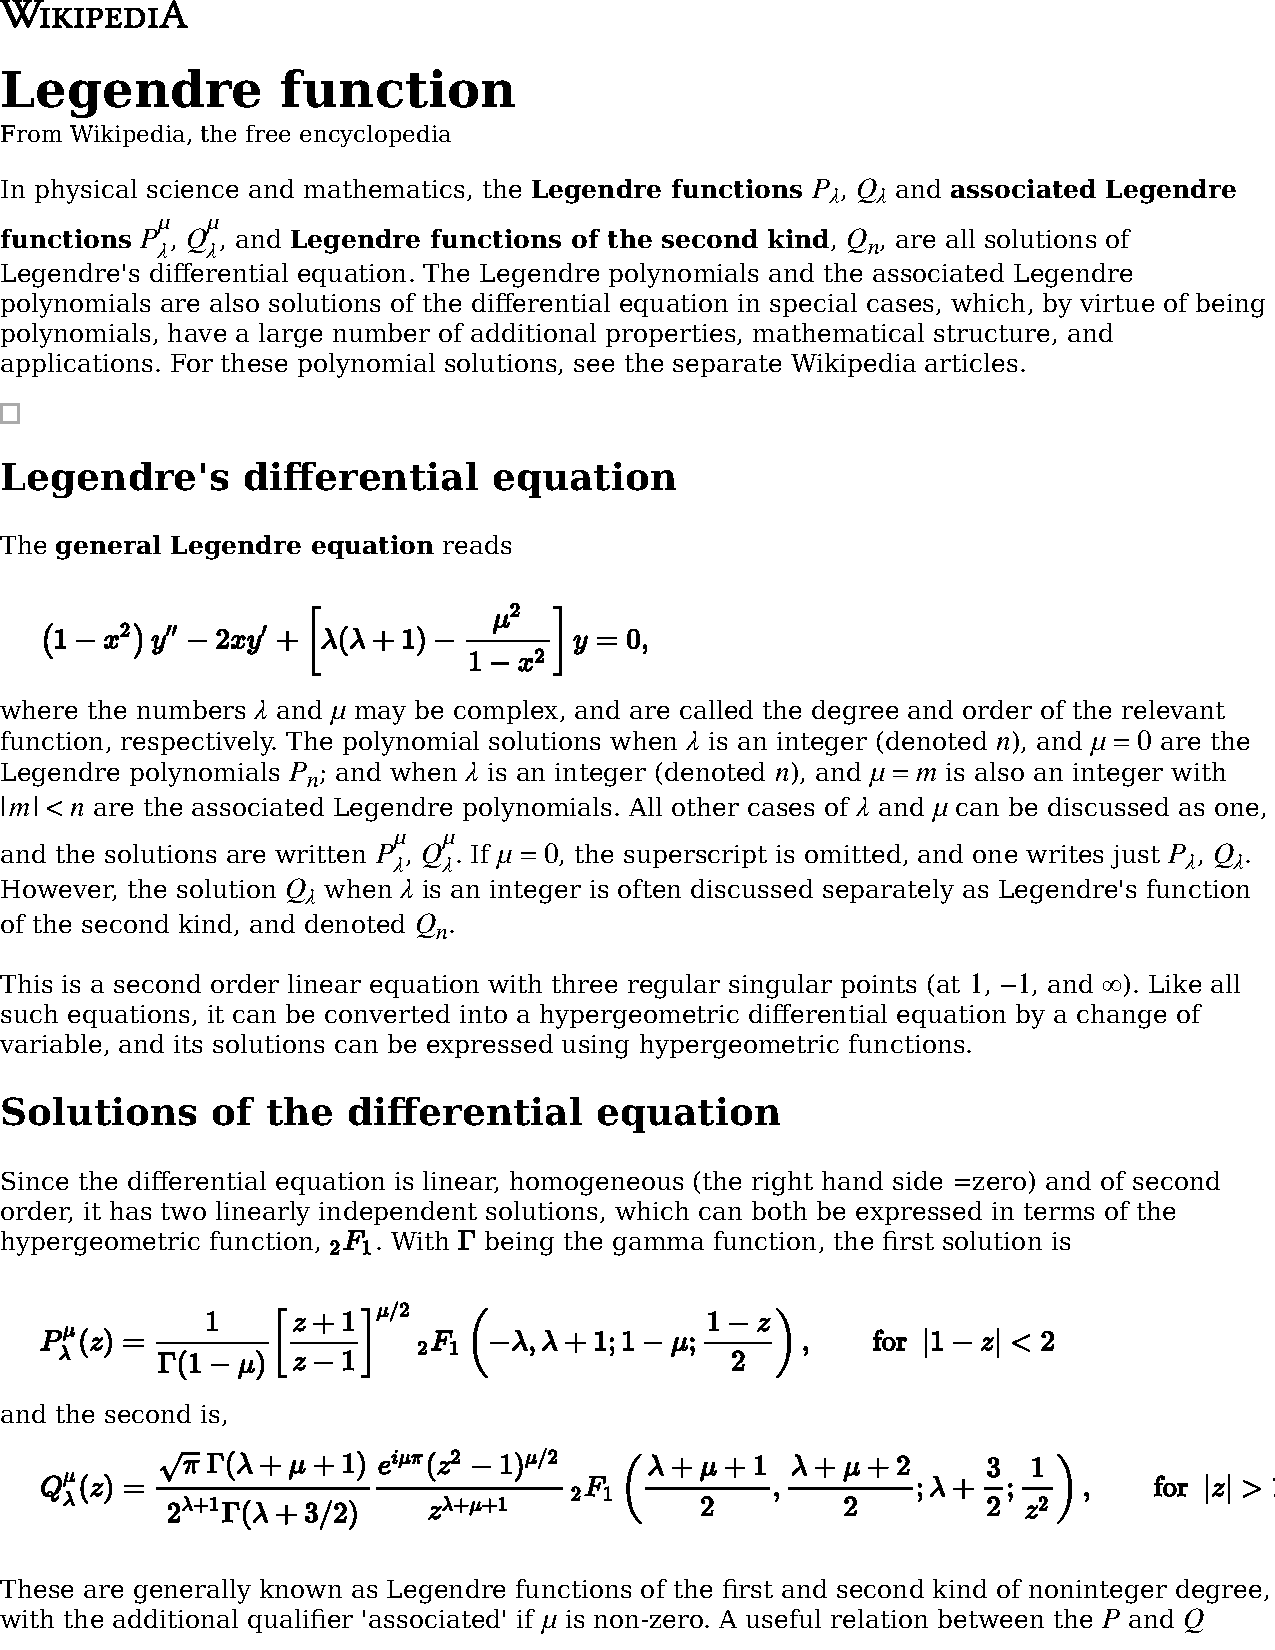
\includegraphics[page=1, clip, trim=0in 3.7in 0in 3.5in, width=\textwidth]{Legendre function - Wikipedia.pdf}
\vfill
Source: Wikipedia, {\it Legendre function}
\end{frame}

\begin{frame}
\frametitle{The radical equation}
Given
\[ \frac{1}{R} \frac{d}{dr}\left[ r^2 \frac{dR}{dr}\right] + 2(Er^2 + r) = l(l+1) \]

if we substitute $R(r) = e^{-r/n} r^l L(r)$, we find:

\[
r \frac{\partial^{2}L}{\partial r^{2}}
+ \left[ 2 \, l + 2 \, - \frac{2 \, r }{n} \right] \frac{\partial L}{\partial r}
+ \left[ 2 \, E r - \frac{2 \, l}{n}
- \frac{2}{n}
+ 2
+ \frac{r }{n^{2}} \right] L
= 0
\]

if $E=-\frac{1}{2n^2}$, then we obtain:

\[
r \frac{\partial^{2}L}{\partial r^{2}}
+ \left[ 2 \, l + 2 \, - \frac{2 \, r }{n} \right] \frac{\partial L}{\partial r}
+ \left[ - \frac{2 \, l}{n}
- \frac{2}{n}
+ 2 \right] L
= 0
\]

changing variables to $\rho = \frac{r}{n}$ and multiplying through by $n$:

\[
\rho \frac{\partial^{2}L}{\partial \rho^{2}}
+ \left[ 2 \, l + 2 \, - 2\rho \right] \frac{\partial L}{\partial \rho}
+ \left[ - 2 \, l - 2 + 2 n \right] L
= 0
\]

\end{frame}


\begin{frame}
\frametitle{The radical equation}
Given
\[ \frac{1}{R} \frac{d}{dr}\left[ r^2 \frac{dR}{dr}\right] + 2(Er^2 + r) = l(l+1) \]

We expand the derivatives and multiply through by $R$ to find:

\[ r^2 \frac{d^2R}{dr^2} + 2r \frac{dR}{dr} + \left[2(E r^2+r) - l(l+1)\right] R = 0 \]

In the limit as $r$ becomes large, this is approximately:

\[ r^2 \frac{d^2R}{dr^2} + 2E r^2 R = 0 \]

\[ \frac{d^2R}{dr^2} + 2E R = 0 \]

suggesting exponential solutions of the form:

\[ R(r) = e^{\pm \sqrt{2E}ir} \]

\end{frame}

\begin{frame}
\frametitle{The radical equation}
Let's flip the sign on $E$, make the substitution $\mu = \sqrt{2E} r$, and write $R(\mu)=e^{-\mu}L(\mu)$:

\[ r^2 \frac{d^2R}{dr^2} + 2r \frac{dR}{dr} + \left[2(-E r^2+r) - l(l+1)\right] R = 0 \]
\end{frame}

\begin{comment}
\begin{frame}
\frametitle{The Generalized Hypergeometric Function}
The ratio of successive terms is:
\[ \frac{c_{k+1}}{c_k} = \frac{(k+a_1)(k+a_2)\cdots(k+a_p)}{(k+b_1)(k+b_2)\cdots(k+b_q)(k+1)} \]

\[ {}_p F_q\left[\genfrac{}{}{0pt}{0}{a_1,a_2,\cdots,a_p}{b_1,b_2,\cdots,b_q};x\right] = \sum_{k=0}^{\infty} c_k x^k \]

Define the differential operator $\delta$:

\[ \delta = z \frac{d}{dz} \]

then

\[ {}_{p+1} F_p\left[\genfrac{}{}{0pt}{0}{a_1,a_2,\cdots,a_{p+1}}{b_1,b_2,\cdots,b_p};x\right] \]

is a solution to the differential equation

\[ \left[ \delta(\delta + b_1 - 1)\cdots(\delta + b_p - 1) - z(\delta+a_1)(\delta+a_2)\cdots(\delta +a_{p+1}) \right] y = 0 \]
\end{frame}
\end{comment}

\begin{frame}
\frametitle{The Classical Solutions to Hydrogen}
\begin{center}
\begin{tabular}{ccc}
{\bf Energy}		& {\bf Wavefunction}		& {\bf Shell} \\
{\bf (Hartrees)}	& & \\
\\
$-\frac{1}{2}$		& $e^{-r}$			& 1s \\
$-\frac{1}{8}$		& $(2-r)e^{-r/2}$		& 2s \\
			& $xe^{-r/2}$			& 2p \\
			& $ye^{-r/2}$			\\
			& $ze^{-r/2}$			\\
$-\frac{1}{18}$		& $(27-18r+2r^2)e^{-r/3}$	& 3s \\
			& $(6-r)xe^{-r/3}$		& 3p \\
			& $(6-r)ye^{-r/3}$		\\
			& $(6-r)ze^{-r/3}$		\\
%%			& $(xy)e^{-r/3}$		& 3d \\
\end{tabular}
\end{center}
\end{frame}

\begin{frame}
\frametitle{The New Solution to Hydrogen}

\[ - \frac{1}{2} \nabla^2 \Psi - \frac{1}{r} \Psi = E \Psi \]

\[ \Psi(x,y,z) = J_0(2\sqrt{x+r}) \]

%% \[ r = \sqrt{x^2+y^2+z^2} \]

\[ E = 0 \]

\vskip 0.5in

$J_0$ is the Bessel function $J_0$

\end{frame}

\begin{frame}
\frametitle{Verification with Mathematica}
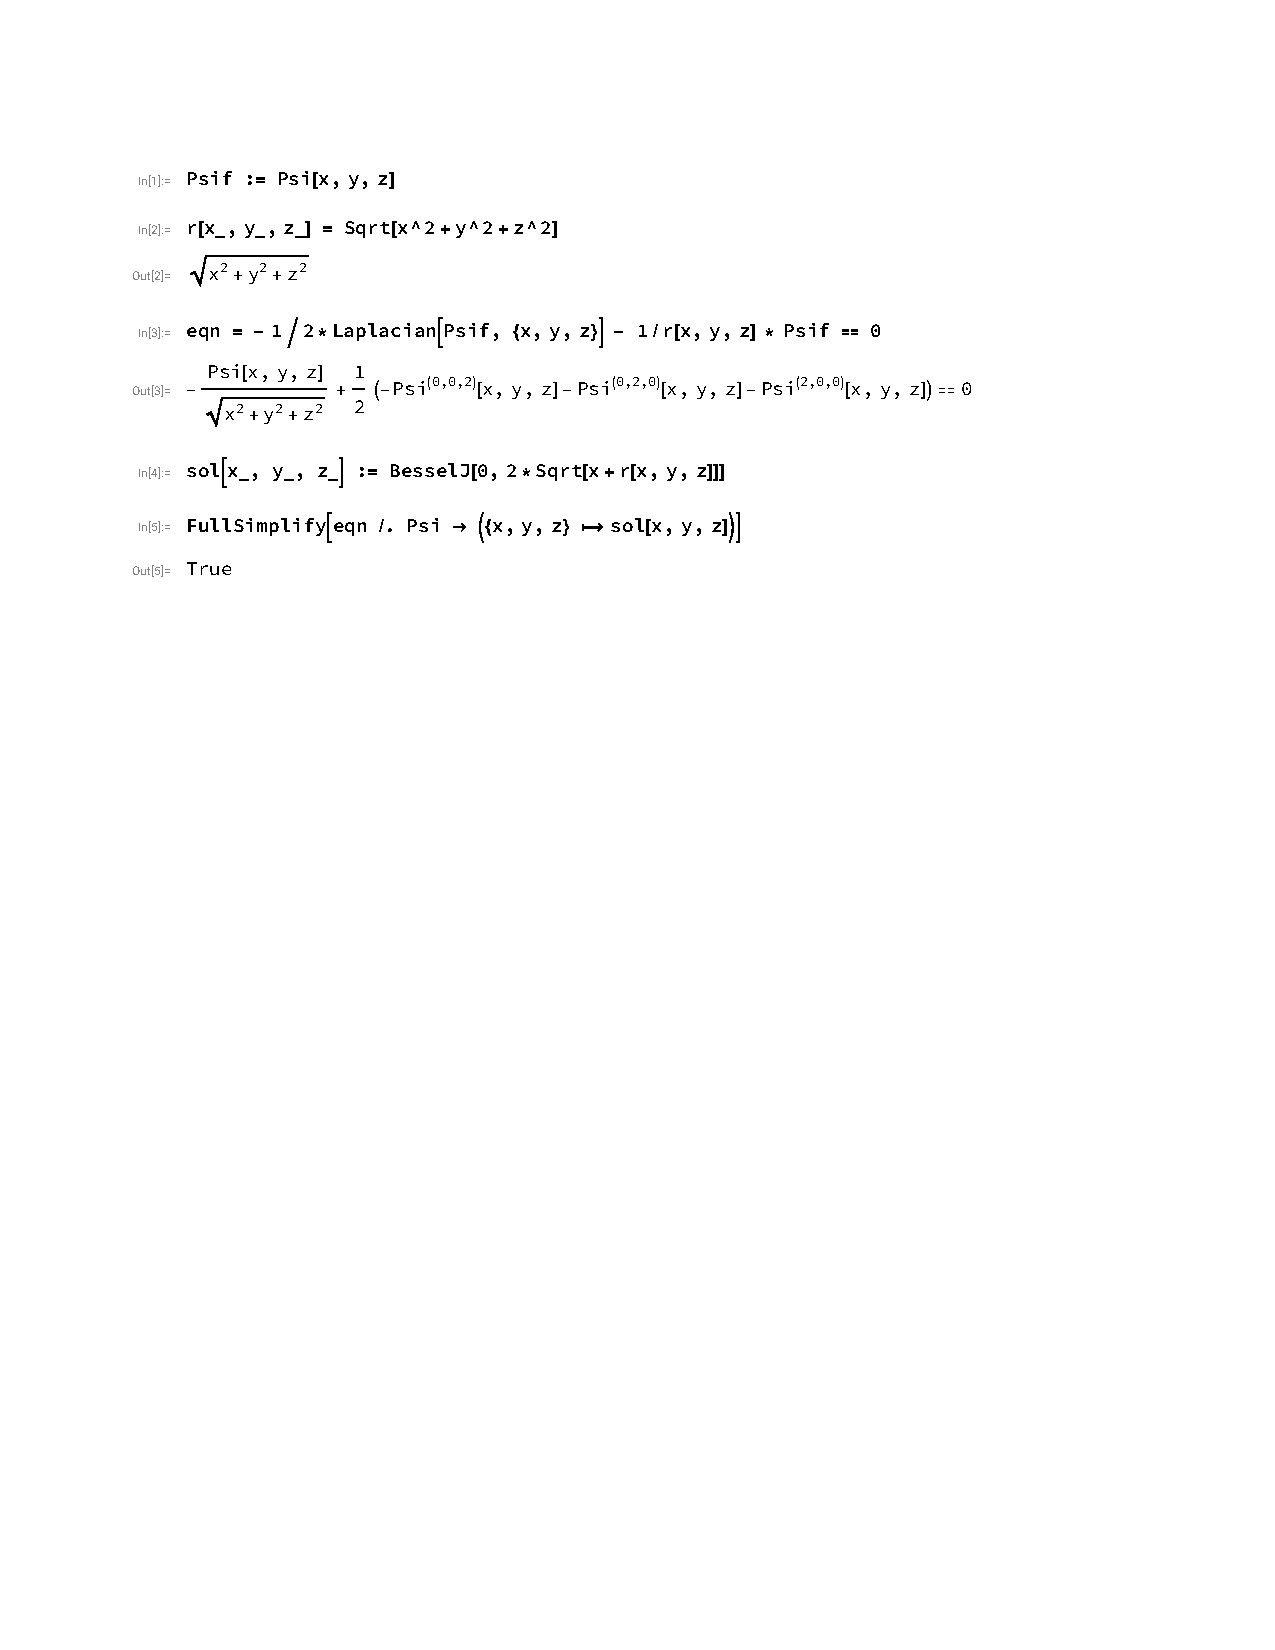
\includegraphics[page=1, clip, trim=1in 7in 1in 1in, width=\textwidth]{improved.pdf}
\end{frame}

%% Add a slide on liouvillian functions

%% Add a slide summarizing the key properties of Bessel functions: ODE, linear ODE, 2nd order, rational coefficients

\begin{frame}
\frametitle{Bessel Functions}
Bessel functions are solutions to the following linear ODE:

\begin{equation}
\label{bessel}
x^2 \frac{d^2 y}{dx^2} + x \frac{dy}{dx} + (x^2 - \alpha^2) y = 0
\end{equation}

The solutions to equation (\ref{bessel}) are not liouvillian.

\vskip 12pt

A second-order linear ODE will have a two dimensional solution space spanned by two linearly independent solutions.

\vskip 12pt

The basis solutions to (\ref{bessel}) are traditionally denoted $J_\alpha$ and $Y_\alpha$.

\vskip 12pt

The general solution to (\ref{bessel}) is:

\[ y(x) = c_0 J_0(x) + c_1 Y_0(x) \qquad c_0,c_1 \in \mathbf{C}\]

$J_\alpha(x)$ is the unique solution to equation (\ref{bessel}) with $J_\alpha(0)=1$

\qquad (integer or positive $\alpha$).

$Y_\alpha(x)$ has a pole at $x=0$, i.e, $\lim_{x\to 0} Y_\alpha(x) = \infty$.
\end{frame}

\begin{frame}
\frametitle{The Bessel functions $J_\alpha(x)$}
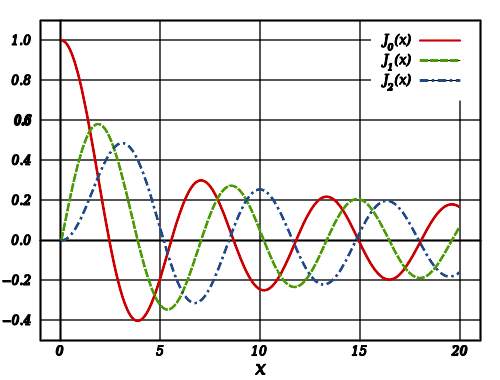
\includegraphics[width=0.9\textwidth]{Bessel_Functions_(1st_Kind,_n=0,1,2).png}
\end{frame}

\begin{frame}
\frametitle{Square Integability of $J_0(2\sqrt{x+r})$}

%% \begin{block}{}
%% For rational $\alpha$, all nonzero roots of $J_\alpha(x)$ are transcendental (Siegel 1929).
%% 
%% \vskip 12pt
%% 
%% The first nonzero root of $J_0(x)$ is approximately 2.40483.
%% 
%% \vskip 12pt
%% Source: Wikipedia, {\it Bessel function}
%% \end{block}

To be a valid wavefunction, $\Psi(x,y,z) = J_0(2\sqrt{x+r})$ must be square integrable:

\[ \int |\Psi|^2\ dV = \int_{-\infty}^{\infty} \int_{-\infty}^{\infty} \int_{-\infty}^{\infty} \left|J_0(2\sqrt{x+r})\right|^2\ dx\ dy\ dz  < \infty\]

Aside: $\int |\Psi|^2\ dV$ is the {\bf L$^2$-norm} of $\psi$.  It shows up a lot.  The L$^2$-norm of
a function is the same as the L$^2$-norm of its Fourier transform, so if the position component of the
wavefunction is square integrable, then the momentum component will also be square integrable.


\end{frame}

\begin{frame}
\frametitle{Square Integability of $J_0(2\sqrt{x+r})$ (cont.)}

Note that $J_0(x) > 0.22$ for all $x<2$:

\begin{block}{}
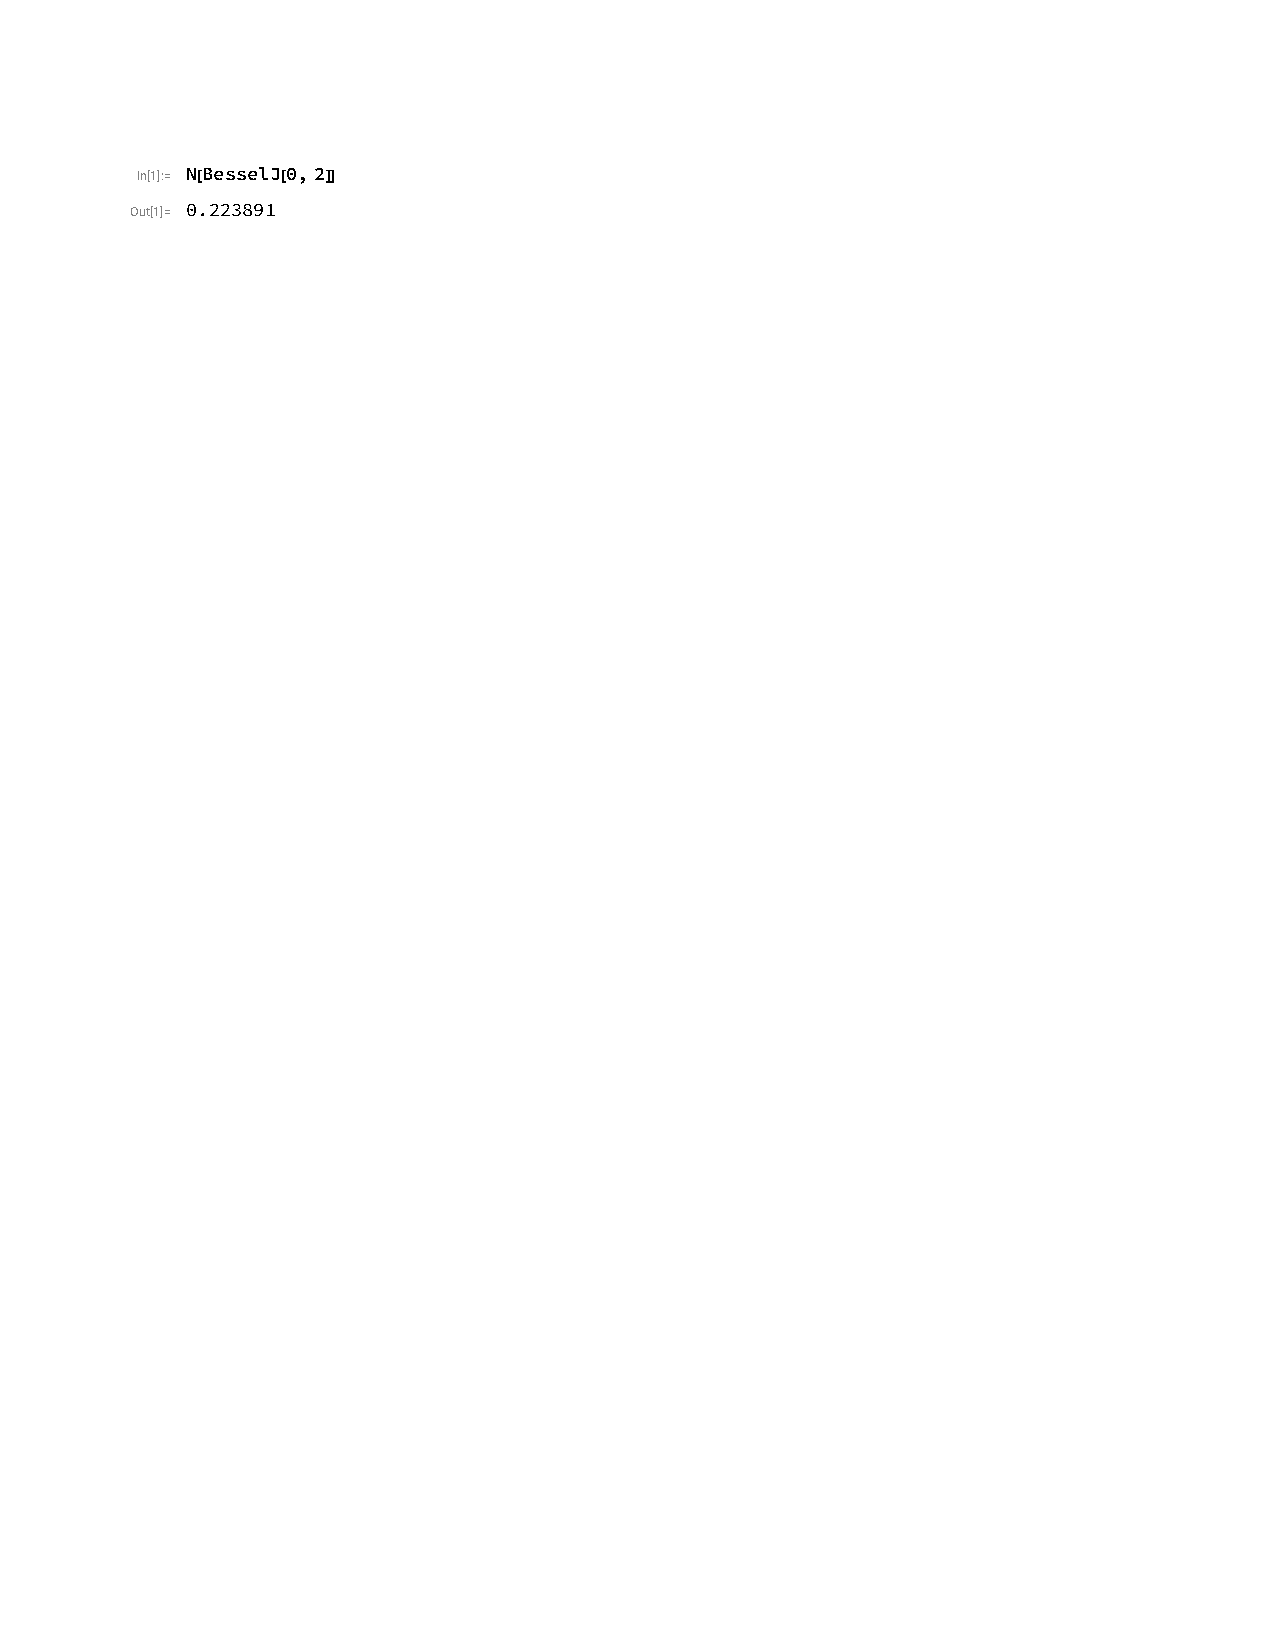
\includegraphics[clip, trim=1in 9.4in 1in 1in, width=\textwidth]{J0-2.pdf}
\end{block}

Consider what happens along the negative $x$-axis: \qquad
\begin{adjustbox}{raise=-.5cm}
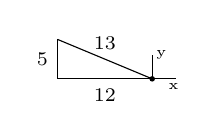
\begin{tikzpicture}[scale=0.1]
\draw (0,0) -- (-12,0) node [pos=0.5, below] {\scriptsize 12};
\draw (-12,0) -- (-12,5) node [pos=0.5, left] {\scriptsize 5};
\draw (0,0) -- (-12,5) node [pos=0.5, above] {\scriptsize 13};

\draw (0,0) -- (3,0) node [pos=0.9, below, yshift=2] {\tiny x};
\draw (0,0) -- (0,3) node [right, xshift=-2] {\tiny y};

\fill (0,0) circle (10pt);
\end{tikzpicture}
\end{adjustbox}

\[ x<-12 \land \sqrt{y^2+z^2} < 5 \Longrightarrow x+r < 1 \Longrightarrow J_0(2\sqrt{x+r}) > 0.22 \]

This implies that the integral of a small block along the negative $x$-axis when $x<-12$ is:

\[ \int_{-1}^{1} \int_{-1}^{1} \int_{x-1}^{x} \left|J_0(2\sqrt{x+r})\right|^2\ dx\ dy\ dz  > 4 \cdot (0.22)^2 \]

Since there are an infinite number of these small blocks, the integral is divergent
and $J_0(2\sqrt{x+r})$ not square integrable.

\end{frame}

\begin{frame}
\begin{exampleblock}{}
\begin{center}
\vskip 20pt
\Huge
Part 2: The solution technique
\vskip 6pt
\ 
\end{center}
\end{exampleblock}
\end{frame}

\begin{frame}
\frametitle{Ansatz 5}

To find the classical solutions to hydrogen, we assumed that the solution was {\it separable}.
This was basically a lucky guess.

\vskip 12pt

Let's make a different assumption (and see if it's lucky, too):

\vskip 12pt

\begin{itemize}
\item The solution satisfies a second-order ODE with rational coefficients

\[ a(v) \frac{d^2 \Psi}{dv^2} + b(v) \frac{d \Psi}{dv} + c(v) \Psi = 0 \]

\item $a(v)$, $b(v)$, $c(v)$ are polynomials in $v$

\item $v$ is a polynomial in $x,y,z,r$

\item $a(v)$, $b(v)$, $c(v)$, and $v$ are all first degree polynomials
\end{itemize}
\end{frame}

\tikzstyle{poly}=[rectangle, draw, thick, fill=white, text width=5em, align=center, rounded corners, minimum height=2em]
\tikzstyle{poly2}=[rectangle, draw, thick, fill=white, align=center, rounded corners, minimum height=2em]
\tikzstyle{ring}=[rectangle, draw=blue, thick, fill=blue!20, text width=5em,align=center, rounded corners, minimum height=2em]
\tikzstyle{element}=[rectangle, draw=orange, thick, fill=orange!20, align=center, rounded corners, minimum height=2em]
\tikzstyle{algebraic}=[rectangle, draw=green, thick, fill=green!20, align=center, rounded corners, minimum height=2em]
\tikzstyle{degree}=[]

\begin{frame}
\frametitle{Ansatz 5}
\begin{center}
  \begin{tikzpicture}[remember picture,out=315,in=225,distance=0.4cm,node distance=40pt]
    \node (Psi) [poly, text width=100pt] {$\framebox(10,10){}\tikzmark{a}\,\Psi'' + \framebox(10,10){}\tikzmark{b}\,\Psi' + \coeff\tikzmark{c}\,\Psi$};
    \node (Qv) [ring, below of=Psi, text width=100pt] {$\mathbf{Q}[v]$};
    \node (v) [poly, right=of Qv] {$v$};
    \draw[degree] (a.west) -- (a.west|-Qv.north) node[right,pos=0.6] {1};
    \draw[degree] (b.west) -- (b.west|-Qv.north) node[right,pos=0.6] {1};
    \draw[degree] (c.west) -- (c.west|-Qv.north) node[right,pos=0.6] {1};
    \node (Psi label) [at=(v.east|-Psi.north), anchor=north east] {\Large$\Psi$};
    \begin{scope}[on background layer]
        \node (Psi block)[fit=(Psi) (Qv) (v), inner sep=10pt, element] {};
    \end{scope}
    \node (base) [ring, node distance=70pt, below=of Psi block.east, anchor=east, text width=250pt] {$\mathbf{Q}[x,y,z,r]/(r^2-x^2-y^2-z^2)$};
    \draw[degree] (v.south) -- (v.south|-base.north) node[right,pos=0.7] {1};
  \end{tikzpicture}
\end{center}

\end{frame}

\begin{frame}
\frametitle{Jet Notation}

\begin{center}
Newton notation: $\Psi''$ or $\ddot \Psi$

\vskip 12pt

Leibnitz notation: $\frac{\delta^2 \Psi(x,y,z)}{\delta x^2}$

\vskip 12pt

Jet notation: $\Psi_{xx}(x,y,z)$ or just $\Psi_{xx}$
\end{center}
\end{frame}

\begin{frame}
\frametitle{Ansatz 5}

\begin{center}

The Hydrogen PDE:

\[ - \frac{1}{2} \Psi_{xx} - \frac{1}{2} \Psi_{yy} - \frac{1}{2} \Psi_{zz} - \frac{1}{r} \Psi = E \Psi \]

\vskip 10pt

Ansatz 5:

\begin{equation*}
\label{ansatz 5a}
v = v_1 x + v_2 y + v_3 z + v_4 r
\end{equation*}

\begin{equation*}
\label{ansatz 5b}
(a_0 + a_1 v) \Psi_{vv} + (b_0 + b_1 v) \Psi_v + (c_0 + c_1 v) \Psi = 0
\end{equation*}

\begin{equation*}
\label{ansatz 5c}
\begin{gathered}
\Psi_x = \Psi_v v_x \qquad
\Psi_y = \Psi_v v_y \qquad
\Psi_z = \Psi_v v_z \\
\Psi_{vx} = \Psi_{vv} v_x \qquad
\Psi_{vy} = \Psi_{vv} v_y \qquad
\Psi_{vz} = \Psi_{vv} v_z \\
\end{gathered}
\end{equation*}

\end{center}

\end{frame}

\begin{frame}
\frametitle{Expansion of $\Psi_{xx}$}

We now substitute ansatz 5 into the hydrogen PDE.

\vskip 12pt

For example, consider the first term in the PDE, $\Psi_{xx}$:

\[ \Psi_{xx} = (\Psi_x)_x = (\Psi_v v_x)_x = \Psi_{vx} v_x + \Psi_v v_{xx} = \Psi_{vv} (v_x)^2 + \Psi_v v_{xx} \]

\[ v_x = \frac{\delta}{\delta x}\left(v_1 x + v_2 y + v_3 z + v_4 r\right) = v_1 + v_4 \frac{x}{r} \]
%% \[ v_{xx} = v_4 \left(\frac{x^2-r^2}{r^3}\right) \]
\[ v_{xx} = v_4 \left(\frac{x^2-r^2}{r^3}\right) = v_4 \left(\frac{-y^2-z^2}{(x^2+y^2+z^2)r}\right) \]

\[ \Psi_{vv} = - \frac{ (b_0 + b_1 v) \Psi_v + (c_0 + c_1 v) \Psi } {a_0 + a_1 v} \]

%%\[ \Psi_{xx} = - \frac{ (b_0 + b_1 v) \Psi_v + (c_0 + c_1 v) \Psi } {a_0 + a_1 v} \left( v_1 + v_4 \frac{x}{r} \right)^2 + v_4 \left(\frac{x^2-r^2}{r^3}\right) \Psi_v \]

\small
\[ \Psi_{xx} = - \frac{ (b_0 + b_1 v) \Psi_v + (c_0 + c_1 v) \Psi } {a_0 + a_1 v} \left( v_1 + v_4 \frac{x}{r} \right)^2 + v_4 \left(\frac{-y^2-z^2}{(x^2+y^2+z^2)r}\right) \Psi_v \]

\end{frame}

\begin{frame}
\frametitle{The Expanded Numerator}
\tiny
\vskip -15pt
\[
\hskip -10pt
\begin{array}{l}
-2 r \Psi x^3 E v_1 a_1-3 r \Psi x^3 v_0^2 v_1 c_1-r \Psi x^3 v_1^3 c_1-r \Psi x^3 v_1 v_2^2 c_1-r \Psi x^3 v_1 v_3^2 c_1-2 r \Psi x^2 y E v_2 a_1-3 r \Psi x^2 y v_0^2 v_2 c_1 \\
-r \Psi x^2 y v_1^2 v_2 c_1-r \Psi x^2 y v_2^3 c_1-r \Psi x^2 y v_2 v_3^2 c_1-2 r \Psi x^2 z E v_3 a_1-3 r \Psi x^2 z v_0^2 v_3 c_1-r \Psi x^2 z v_1^2 v_3 c_1-r \Psi x^2 z v_2^2 v_3 c_1 \\
-r \Psi x^2 z v_3^3 c_1
-2 r \Psi x^2 E a_0-r \Psi x^2 v_0^2 c_0-2 r \Psi x^2 v_0 a_1-r \Psi x^2 v_1^2 c_0-r \Psi x^2 v_2^2 c_0-r \Psi x^2 v_3^2 c_0-2 r \Psi x y^2 E v_1 a_1 \\
-3 r \Psi x y^2 v_0^2 v_1 c_1
-r \Psi x y^2 v_1^3 c_1
-r \Psi x y^2 v_1 v_2^2 c_1-r \Psi x y^2 v_1 v_3^2 c_1-2 r \Psi x z^2 E v_1 a_1-3 r \Psi x z^2 v_0^2 v_1 c_1-r \Psi x z^2 v_1^3 c_1 \\
-r \Psi x z^2 v_1 v_2^2 c_1
-r \Psi x z^2 v_1 v_3^2 c_1-2 r \Psi y^3 E v_2 a_1
-3 r \Psi y^3 v_0^2 v_2 c_1-r \Psi y^3 v_1^2 v_2 c_1-r \Psi y^3 v_2^3 c_1-r \Psi y^3 v_2 v_3^2 c_1
-2 r \Psi y^2 z E v_3 a_1
\\
-3 r \Psi y^2 z v_0^2 v_3 c_1-r \Psi y^2 z v_1^2 v_3 c_1-r \Psi y^2 z v_2^2 v_3 c_1
-r \Psi y^2 z v_3^3 c_1-2 r \Psi y^2 E a_0
-r \Psi y^2 v_0^2 c_0-2 r \Psi y^2 v_0 a_1-r \Psi y^2 v_1^2 c_0
\\
-r \Psi y^2 v_2^2 c_0-r \Psi y^2 v_3^2 c_0-2 r \Psi y z^2 E v_2 a_1 -3 r \Psi y z^2 v_0^2 v_2 c_1
-r \Psi y z^2 v_1^2 v_2 c_1-r \Psi y z^2 v_2^3 c_1-r \Psi y z^2 v_2 v_3^2 c_1-2 r \Psi z^3 E v_3 a_1
\\
-3 r \Psi z^3 v_0^2 v_3 c_1-r \Psi z^3 v_1^2 v_3 c_1-r \Psi z^3 v_2^2 v_3 c_1-r \Psi z^3 v_3^3 c_1-2 r \Psi z^2 E a_0
-r \Psi z^2 v_0^2 c_0-2 r \Psi z^2 v_0 a_1-r \Psi z^2 v_1^2 c_0
\\
-r \Psi z^2 v_2^2 c_0
-r \Psi z^2 v_3^2 c_0
-3 r \Psi_v x^3 v_0^2 v_1 b_1-r \Psi_v x^3 v_1^3 b_1-r \Psi_v x^3 v_1 v_2^2 b_1-r \Psi_v x^3 v_1 v_3^2 b_1
-3 r \Psi_v x^2 y v_0^2 v_2 b_1
\\
-r \Psi_v x^2 y v_1^2 v_2 b_1-r \Psi_v x^2 y v_2^3 b_1-r \Psi_v x^2 y v_2 v_3^2 b_1-3 r \Psi_v x^2 z v_0^2 v_3 b_1-r \Psi_v x^2 z v_1^2 v_3 b_1-r \Psi_v x^2 z v_2^2 v_3 b_1
-2 r \Psi_v y^2 v_0^2 a_1 \\
-r \Psi_v x^2 z v_3^3 b_1-2 r \Psi_v x^2 v_0^2 a_1-r \Psi_v x^2 v_0^2 b_0-r \Psi_v x^2 v_1^2 b_0-r \Psi_v x^2 v_2^2 b_0-r \Psi_v x^2 v_3^2 b_0-3 r \Psi_v x y^2 v_0^2 v_1 b_1-r \Psi_v x y^2 v_1^3 b_1 \\
-r \Psi_v x y^2 v_1 v_2^2 b_1
-r \Psi_v x y^2 v_1 v_3^2 b_1-3 r \Psi_v x z^2 v_0^2 v_1 b_1-r \Psi_v x z^2 v_1^3 b_1-r \Psi_v x z^2 v_1 v_2^2 b_1-r \Psi_v x z^2 v_1 v_3^2 b_1
-3 r \Psi_v y^3 v_0^2 v_2 b_1 \\
-r \Psi_v y^3 v_1^2 v_2 b_1-r \Psi_v y^3 v_2^3 b_1-r \Psi_v y^3 v_2 v_3^2 b_1-3 r \Psi_v y^2 z v_0^2 v_3 b_1-r \Psi_v y^2 z v_1^2 v_3 b_1-r \Psi_v y^2 z v_2^2 v_3 b_1-r \Psi_v y^2 z v_3^3 b_1 \\
-r \Psi_v y^2 v_0^2 b_0-r \Psi_v y^2 v_1^2 b_0-r \Psi_v y^2 v_2^2 b_0-r \Psi_v y^2 v_3^2 b_0-3 r \Psi_v y z^2 v_0^2 v_2 b_1-r \Psi_v y z^2 v_1^2 v_2 b_1-r \Psi_v y z^2 v_2^3 b_1
\\
-3 r \Psi_v z^3 v_0^2 v_3 b_1-r \Psi_v z^3 v_1^2 v_3 b_1-r \Psi_v z^3 v_2^2 v_3 b_1-r \Psi_v z^3 v_3^3 b_1-2 r \Psi_v z^2 v_0^2 a_1-r \Psi_v z^2 v_0^2 b_0-r \Psi_v z^2 v_1^2 b_0-r \Psi_v z^2 v_2^2 b_0 \\
-r \Psi_v z^2 v_3^2 b_0-2 \Psi x^4 E v_0 a_1-\Psi x^4 v_0^3 c_1-3 \Psi x^4 v_0 v_1^2 c_1-\Psi x^4 v_0 v_2^2 c_1-\Psi x^4 v_0 v_3^2 c_1-4 \Psi x^3 y v_0 v_1 v_2 c_1-4 \Psi x^3 z v_0 v_1 v_3 c_1 \\
-2 \Psi x^3 v_0 v_1 c_0-2 \Psi x^3 v_1 a_1-4 \Psi x^2 y^2 E v_0 a_1-2 \Psi x^2 y^2 v_0^3 c_1-4 \Psi x^2 y^2 v_0 v_1^2 c_1-4 \Psi x^2 y^2 v_0 v_2^2 c_1
-2 \Psi x^2 y^2 v_0 v_3^2 c_1
\\
-4 \Psi x^2 y z v_0 v_2 v_3 c_1-2 \Psi x^2 y v_0 v_2 c_0-2 \Psi x^2 y v_2 a_1-4 \Psi x^2 z^2 E v_0 a_1-2 \Psi x^2 z^2 v_0^3 c_1
-4 \Psi x^2 z^2 v_0 v_1^2 c_1-2 \Psi x^2 z^2 v_0 v_2^2 c_1
\\
-4 \Psi x^2 z^2 v_0 v_3^2 c_1
-2 \Psi x^2 z v_0 v_3 c_0-2 \Psi x^2 z v_3 a_1-2 \Psi x^2 a_0-4 \Psi x y^3 v_0 v_1 v_2 c_1-4 \Psi x y^2 z v_0 v_1 v_3 c_1-2 \Psi x y^2 v_0 v_1 c_0
\\
-2 \Psi x y^2 v_1 a_1-4 \Psi x y z^2 v_0 v_1 v_2 c_1-4 \Psi x z^3 v_0 v_1 v_3 c_1-2 \Psi x z^2 v_0 v_1 c_0-2 \Psi x z^2 v_1 a_1-2 \Psi y^4 E v_0 a_1-\Psi y^4 v_0^3 c_1
-\Psi y^4 v_0 v_1^2 c_1
\\
-3 \Psi y^4 v_0 v_2^2 c_1-\Psi y^4 v_0 v_3^2 c_1-4 \Psi y^3 z v_0 v_2 v_3 c_1-2 \Psi y^3 v_0 v_2 c_0-2 \Psi y^3 v_2 a_1-4 \Psi y^2 z^2 E v_0 a_1-2 \Psi y^2 z^2 v_0^3 c_1
-r \Psi_v y z^2 v_2 v_3^2 b_1 \\
-2 \Psi y^2 z^2 v_0 v_1^2 c_1-4 \Psi y^2 z^2 v_0 v_2^2 c_1-4 \Psi y^2 z^2 v_0 v_3^2 c_1-2 \Psi y^2 z v_0 v_3 c_0-2 \Psi y^2 z v_3 a_1-2 \Psi y^2 a_0-4 \Psi y z^3 v_0 v_2 v_3 c_1
\\
-2 \Psi y z^2 v_0 v_2 c_0-2 \Psi y z^2 v_2 a_1-2 \Psi z^4 E v_0 a_1-\Psi z^4 v_0^3 c_1-\Psi z^4 v_0 v_1^2 c_1-\Psi z^4 v_0 v_2^2 c_1-3 \Psi z^4 v_0 v_3^2 c_1-2 \Psi z^3 v_0 v_3 c_0
\\
-2 \Psi z^3 v_3 a_1-2 \Psi z^2 a_0-\Psi_v x^4 v_0^3 b_1-3 \Psi_v x^4 v_0 v_1^2 b_1-\Psi_v x^4 v_0 v_2^2 b_1-\Psi_v x^4 v_0 v_3^2 b_1-4 \Psi_v x^3 y v_0 v_1 v_2 b_1-4 \Psi_v x^3 z v_0 v_1 v_3 b_1
\\
-2 \Psi_v x^3 v_0 v_1 a_1-2 \Psi_v x^3 v_0 v_1 b_0-2 \Psi_v x^2 y^2 v_0^3 b_1-4 \Psi_v x^2 y^2 v_0 v_1^2 b_1-4 \Psi_v x^2 y^2 v_0 v_2^2 b_1-2 \Psi_v x^2 y^2 v_0 v_3^2 b_1
\\
-4 \Psi_v x^2 y z v_0 v_2 v_3 b_1-2 \Psi_v x^2 y v_0 v_2 a_1-2 \Psi_v x^2 y v_0 v_2 b_0-2 \Psi_v x^2 z^2 v_0^3 b_1-4 \Psi_v x^2 z^2 v_0 v_1^2 b_1-2 \Psi_v x^2 z^2 v_0 v_2^2 b_1
\\
-2 \Psi_v x^2 z v_0 v_3 a_1-2 \Psi_v x^2 z v_0 v_3 b_0-2 \Psi_v x^2 v_0 a_0-4 \Psi_v x y^3 v_0 v_1 v_2 b_1-4 \Psi_v x y^2 z v_0 v_1 v_3 b_1-2 \Psi_v x y^2 v_0 v_1 a_1-4 \Psi_v x^2 z^2 v_0 v_3^2 b_1
\\
-2 \Psi_v x y^2 v_0 v_1 b_0-4 \Psi_v x y z^2 v_0 v_1 v_2 b_1-4 \Psi_v x z^3 v_0 v_1 v_3 b_1-2 \Psi_v x z^2 v_0 v_1 a_1-2 \Psi_v x z^2 v_0 v_1 b_0-\Psi_v y^4 v_0^3 b_1-\Psi_v y^4 v_0 v_1^2 b_1
\\
-3 \Psi_v y^4 v_0 v_2^2 b_1-\Psi_v y^4 v_0 v_3^2 b_1-4 \Psi_v y^3 z v_0 v_2 v_3 b_1-2 \Psi_v y^3 v_0 v_2 a_1-2 \Psi_v y^3 v_0 v_2 b_0-2 \Psi_v y^2 z^2 v_0^3 b_1-2 \Psi_v y^2 z^2 v_0 v_1^2 b_1
\\
-4 \Psi_v y^2 z^2 v_0 v_2^2 b_1-4 \Psi_v y^2 z^2 v_0 v_3^2 b_1-2 \Psi_v y^2 z v_0 v_3 a_1-2 \Psi_v y^2 z v_0 v_3 b_0-2 \Psi_v y^2 v_0 a_0-4 \Psi_v y z^3 v_0 v_2 v_3 b_1-2 \Psi_v y z^2 v_0 v_2 a_1
\\
-2 \Psi_v y z^2 v_0 v_2 b_0-\Psi_v z^4 v_0^3 b_1-\Psi_v z^4 v_0 v_1^2 b_1-\Psi_v z^4 v_0 v_2^2 b_1-3 \Psi_v z^4 v_0 v_3^2 b_1-2 \Psi_v z^3 v_0 v_3 a_1-2 \Psi_v z^3 v_0 v_3 b_0-2 \Psi_v z^2 v_0 a_0
\end{array}
\]
\end{frame}

\begin{frame}
\frametitle{Collect Like Terms}
Collect like terms in $\Psi$, $\Psi_v$, $x$, $y$, $z$, and $r$.

\[ r\Psi x^3 \left(-2 E a_1 v_1 - 3 c_1 v_0^2 v_1 - c_1 v_1^3 - c_1 v_1 v_2^2 - c_1 v_1 v_3^2\right) - \cdots \]
\end{frame}

\begin{frame}
\frametitle{The System of Equations}
%%\scriptsize
\fontsize{9}{11}\selectfont
\begin{minipage}{.7\linewidth}
\begin{equation*}
\begin{array}{r}
-2 \, c_{1} v_{0}^{3} - 4 \, c_{1} v_{0} v_{1}^{2} - 4 \, c_{1} v_{0} v_{2}^{2} - 2 \, c_{1} v_{0} v_{3}^{2} - 4 \, E a_{1} v_{0} =0\\
-2 \, c_{1} v_{0}^{3} - 4 \, c_{1} v_{0} v_{1}^{2} - 2 \, c_{1} v_{0} v_{2}^{2} - 4 \, c_{1} v_{0} v_{3}^{2} - 4 \, E a_{1} v_{0} =0\\
-2 \, c_{1} v_{0}^{3} - 2 \, c_{1} v_{0} v_{1}^{2} - 4 \, c_{1} v_{0} v_{2}^{2} - 4 \, c_{1} v_{0} v_{3}^{2} - 4 \, E a_{1} v_{0} =0\\
-3 \, b_{1} v_{0}^{2} v_{1} -  \, b_{1} v_{1}^{3} -  \, b_{1} v_{1} v_{2}^{2} -  \, b_{1} v_{1} v_{3}^{2} =0\\
-3 \, b_{1} v_{0}^{2} v_{2} -  \, b_{1} v_{1}^{2} v_{2} -  \, b_{1} v_{2}^{3} -  \, b_{1} v_{2} v_{3}^{2} =0\\
-3 \, b_{1} v_{0}^{2} v_{3} -  \, b_{1} v_{1}^{2} v_{3} -  \, b_{1} v_{2}^{2} v_{3} -  \, b_{1} v_{3}^{3} =0\\
-2 \, b_{1} v_{0}^{3} - 4 \, b_{1} v_{0} v_{1}^{2} - 4 \, b_{1} v_{0} v_{2}^{2} - 2 \, b_{1} v_{0} v_{3}^{2} =0\\
-2 \, b_{1} v_{0}^{3} - 4 \, b_{1} v_{0} v_{1}^{2} - 2 \, b_{1} v_{0} v_{2}^{2} - 4 \, b_{1} v_{0} v_{3}^{2} =0\\
-3 \, c_{1} v_{0}^{2} v_{1} -  \, c_{1} v_{1}^{3} -  \, c_{1} v_{1} v_{2}^{2} -  \, c_{1} v_{1} v_{3}^{2} - 2 \, E a_{1} v_{1} =0\\
-3 \, c_{1} v_{0}^{2} v_{2} -  \, c_{1} v_{1}^{2} v_{2} -  \, c_{1} v_{2}^{3} -  \, c_{1} v_{2} v_{3}^{2} - 2 \, E a_{1} v_{2} =0\\
-3 \, c_{1} v_{0}^{2} v_{3} -  \, c_{1} v_{1}^{2} v_{3} -  \, c_{1} v_{2}^{2} v_{3} -  \, c_{1} v_{3}^{3} - 2 \, E a_{1} v_{3} =0\\
-2 \, b_{1} v_{0}^{3} - 2 \, b_{1} v_{0} v_{1}^{2} - 4 \, b_{1} v_{0} v_{2}^{2} - 4 \, b_{1} v_{0} v_{3}^{2} =0\\
- \, c_{0} v_{0}^{2} -  \, c_{0} v_{1}^{2} -  \, c_{0} v_{2}^{2} -  \, c_{0} v_{3}^{2} - 2 \, E a_{0} - 2 \, a_{1} v_{0} =0\\
- \, c_{1} v_{0}^{3} - 3 \, c_{1} v_{0} v_{1}^{2} -  \, c_{1} v_{0} v_{2}^{2} -  \, c_{1} v_{0} v_{3}^{2} - 2 \, E a_{1} v_{0} =0\\
- \, c_{1} v_{0}^{3} -  \, c_{1} v_{0} v_{1}^{2} - 3 \, c_{1} v_{0} v_{2}^{2} -  \, c_{1} v_{0} v_{3}^{2} - 2 \, E a_{1} v_{0} =0\\
- \, c_{1} v_{0}^{3} -  \, c_{1} v_{0} v_{1}^{2} -  \, c_{1} v_{0} v_{2}^{2} - 3 \, c_{1} v_{0} v_{3}^{2} - 2 \, E a_{1} v_{0} =0\\
-2 \, a_{1} v_{0}^{2} -  \, b_{0} v_{0}^{2} -  \, b_{0} v_{1}^{2} -  \, b_{0} v_{2}^{2} -  \, b_{0} v_{3}^{2} =0\\
- \, b_{1} v_{0}^{3} - 3 \, b_{1} v_{0} v_{1}^{2} -  \, b_{1} v_{0} v_{2}^{2} -  \, b_{1} v_{0} v_{3}^{2} =0\\
- \, b_{1} v_{0}^{3} -  \, b_{1} v_{0} v_{1}^{2} - 3 \, b_{1} v_{0} v_{2}^{2} -  \, b_{1} v_{0} v_{3}^{2} =0\\
- \, b_{1} v_{0}^{3} -  \, b_{1} v_{0} v_{1}^{2} -  \, b_{1} v_{0} v_{2}^{2} - 3 \, b_{1} v_{0} v_{3}^{2} =0
\end{array}
\end{equation*}
\end{minipage}%
\begin{minipage}{.3\linewidth}
\begin{equation*}
\begin{array}{r}
-4 \, b_{1} v_{0} v_{1} v_{2} =0\\
-4 \, b_{1} v_{0} v_{1} v_{3} =0\\
-4 \, b_{1} v_{0} v_{2} v_{3} =0\\
-4 \, c_{1} v_{0} v_{1} v_{2} =0\\
-4 \, c_{1} v_{0} v_{1} v_{3} =0\\
-4 \, c_{1} v_{0} v_{2} v_{3} =0\\
-2 \, c_{0} v_{0} v_{1} - 2 \, a_{1} v_{1} =0\\
-2 \, c_{0} v_{0} v_{2} - 2 \, a_{1} v_{2} =0\\
-2 \, c_{0} v_{0} v_{3} - 2 \, a_{1} v_{3} =0\\
-2 \, a_{1} v_{0} v_{1} - 2 \, b_{0} v_{0} v_{1} =0\\
-2 \, a_{1} v_{0} v_{2} - 2 \, b_{0} v_{0} v_{2} =0\\
-2 \, a_{1} v_{0} v_{3} - 2 \, b_{0} v_{0} v_{3} =0\\
-2 \, a_{0} =0\\
-2 \, a_{0} v_{0} =0\\
\end{array}
\end{equation*}
\end{minipage}
\end{frame}

\begin{frame}
\frametitle{Rings, Ideals and Varieties}
\begin{definition}[commutative algebra]
A {\it commutative ring} is a set of objects closed under two binary operations, addition and multiplication,
that satisfies the following axioms:
\end{definition}

\begin{definition}[commutative algebra]
An {\it ideal} $I$ of a ring $R$ is a subring of $R$ closed under multiplication with elements from $R$:
\[ \forall r \in R, \forall a \in I, ra \in I \]
\end{definition}

\begin{definition}[algebraic geometry]
An {\it algebraic variety} $V$ is the zero locus of some set of polynomials $S$:
\[ V(S) = \{ x \in {\mathbb A}^n | f(x) = 0 \quad\forall f \in S \} \]
\end{definition}
\end{frame}

\begin{frame}
\frametitle{Radical Ideals}
\begin{definition}[commutative algebra]
The {\it radical} of an ideal $I$ of a ring $R$ is:
\[ \sqrt{I} = \{ a \in R \ | \ \exists n \in {\mathbb Z}, a^n \in I \} \]
\end{definition}
\end{frame}

\begin{frame}[fragile]
\frametitle{The Prime Decomposition of the System of Equations}
\begin{verbatim}
sage: I.radical().primary_decomposition()
\end{verbatim}

\begin{subequations}
\label{ideal}
\begin{align}
& \left(n_{1}, n_{0}, m_{1}, m_{0}, d_{1}, d_{0}\right)\label{ideal:5} \\
& \qquad \text{sets all coefficients of the ODE to zero} \nonumber \\
& \left(v_{3}, v_{2}, v_{1}, v_{0}, d_{0}\right)\label{ideal:4}\\
& \qquad \text{sets the variable $v$ to zero} \nonumber \\
& \left(v_{1}^{2} + v_{2}^{2} + v_{3}^{2}, v_{0}, d_{1}, d_{0}\right)\label{ideal:3}\\
& \qquad \text{sets the coefficient of $\Psi_{vv}$ in the ODE to zero} \nonumber \\
& \left(v_{3}, v_{2}, v_{1}, m_{1}, m_{0} - n_{0} v_{0}, 2 d_{1} + n_{0} v_{0}, d_{0}, E n_{0} - n_{1} v_{0}\right)\label{ideal:2}\\
& \qquad \text{the classical solution} \nonumber \\
& \left(v_{0}^{2} - v_{1}^{2} - v_{2}^{2} - v_{3}^{2}, n_{1}, m_{1}, m_{0} - n_{0} v_{0}, d_{1} + n_{0} v_{0}, d_{0}, E\right)\label{ideal:1}\\
& \qquad \text{the new solution} \nonumber
\end{align}
\end{subequations}
\end{frame}

\begin{frame}
\frametitle{Ideal \eqref{ideal:2}}
\[ \left(v_{3}, v_{2}, v_{1}, b_{1}, b_{0} - c_{0} v_{0}, 2 a_{1} + c_{0} v_{0}, a_{0}, E c_{0} - c_{1} v_{0}\right) \]

%% $a_0$ is an ideal generator, so $a_0=0$

We can always multiply our homogenous differential polynomial by a constant without affecting our result, so we can set $a_1=1$.

Likewise, we can multiply our variable $v$ by a constant and that will only change our coefficients by constants,
so set $v_0=1$.
% so we can normalize by setting $v_0=1$.
% and $v_1=v_2=v_3=0$, so we can normalize by setting $v_0=1$.  This simplifies ideal \eqref{ideal:2} to:

\begin{equation*}
\left(v_{3}, v_{2}, v_{1}, v_{0} - 1, c_{0} + 2, b_{1}, b_{0} + 2, a_{1} - 1, a_{0}, 2 E + c_{1}\right)
\end{equation*}

\begin{equation*}
\label{classical eq in ideal}
\begin{gathered}
v=r \\
v \Psi'' + 2 \Psi' + 2(1 + E v) \Psi = 0
\end{gathered}
\end{equation*}

This is the classical radial equation obtained by seperation of variables,
with the orbital quantum number $l=0$,
though it is more commonly written in this form:

\begin{equation*}
\frac{1}{R} \frac{d}{dr}\left[ r^2 \frac{dR}{dr}\right] + 2(Er^2 + r) = 0
\end{equation*}
\end{frame}

\begin{frame}
\frametitle{Ideal \eqref{ideal:1}}
Ideal \eqref{ideal:1} was not expected, and contains our new solution.
$a_0$ is an ideal generator,
so $a_0=0$, and we can set $a_1=1$, by the same logic as above.
Our coordinates are in real space, so our $v_i$ coefficients must be real (why?), so all of their squares must
be positive, and since $v_0^2-v_1^2-v_2^2-v_3^3=0$, $v_0$ must be non-zero.  So we can normalize by setting $v_0=1$.
That simplifies \eqref{ideal:1} to this ideal:

\begin{equation}
\left(v_{1}^{2} + v_{2}^{2} + v_{3}^{2} - 1, v_{0} - 1, c_{1}, c_{0} + 1, b_{1}, b_{0} + 1, a_{1} - 1, a_{0}, E\right)
\end{equation}

This ideal corresponds to the following system of equations:

\begin{equation}
\begin{gathered}
E = 0 \\
a_0 = 0 \qquad
a_1 = 1 \\
b_0 = -1 \qquad
b_1 = 0 \\
c_0 = -1 \qquad
n_1 = 0 \\
v_0 = 1 \qquad
v_1^2 + v_2^2 + v_3^2 = 1
\end{gathered}
\end{equation}

\end{frame}

\begin{frame}
\frametitle{Ideal \eqref{ideal:1} (cont)}

Substituting these values back into our ansatz, we conclude that $\Psi(v)$
is a solution of \eqref{schrodinger} under these conditions:

\begin{equation}
\label{related solution}
\begin{gathered}
v \frac{\delta^2\Psi}{\delta v^2} + \frac{\delta\Psi}{\delta v} + \Psi = 0 \\
v = v_1 x+ v_2 y+ v_3 z+r \\
v_1^2 + v_2^2 + v_3^2 = 1
\end{gathered}
\end{equation}

The expression $v_1 x + v_2 y + v_3 z$ is easily identified as a dot product between
the coordinate $(x,y,z)$ and the unit vector $(v_1, v_2, v_3)$ (remembering
that $v_1^2 + v_2^2 + v_3^2 = 1$).  The direction of this vector is arbitrary,
so we can orient the $x$-axis in this direction and set $(v_1, v_2, v_3) = (1,0,0)$
without loss of generality.

We now have to solve a second order ODE:

\begin{equation}
v \Psi''(v) + \Psi'(v) + \Psi(v) = 0
\end{equation}

\end{frame}

\begin{frame}
\frametitle{Ideal \eqref{ideal:1} (cont)}

Wolfram Mathematica can now
analyze this equation and determine that it can be solved with Bessel functions:

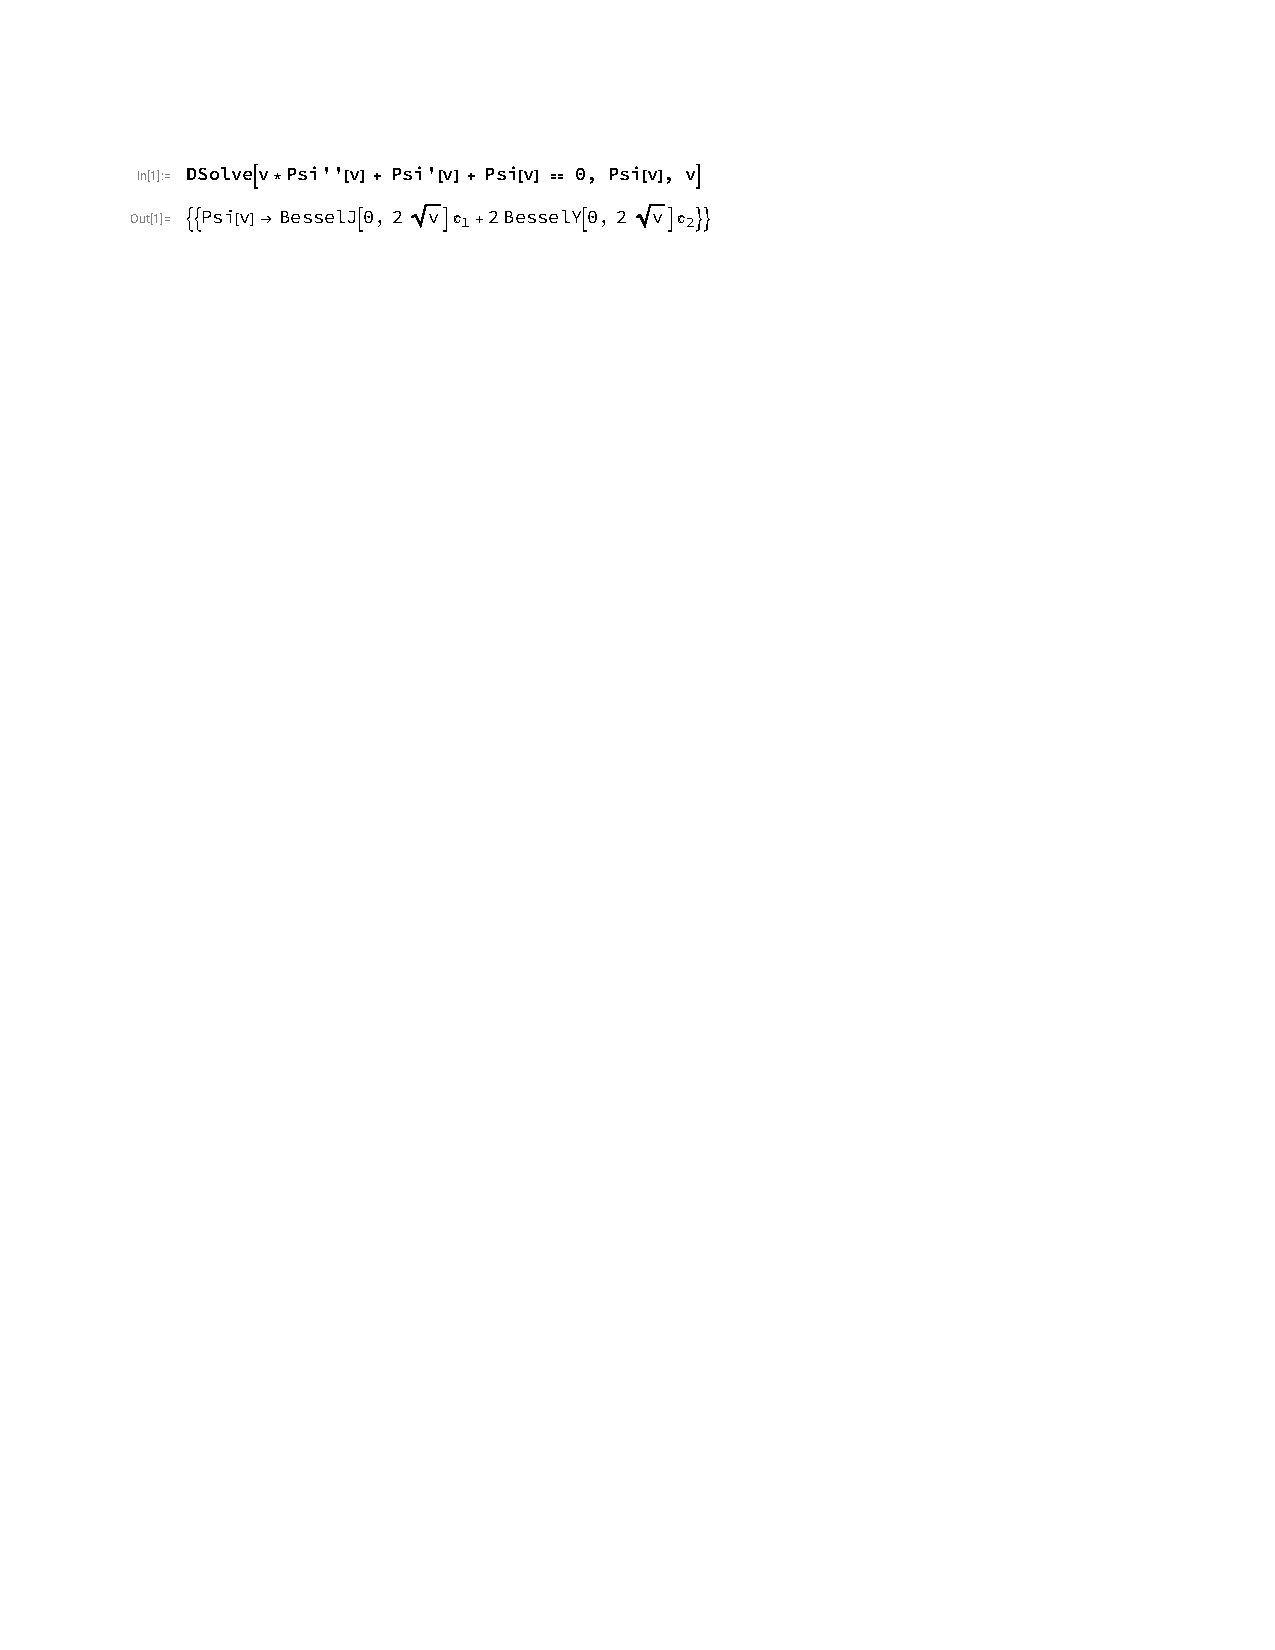
\includegraphics[page=1, clip, trim=1in 9in 1in 0.5in, width=\textwidth]{find Bessel solution.pdf}

{\tt BesselY} is a Bessel function of the second kind.  It has a singularity at $x=0$ and is also not square integrable.

\vskip 12pt

Plugging in $v=x+r$, we obtain:

\[ \psi(x,y,z) = J_0(2\sqrt{x+r}) \]
\end{frame}

\begin{frame}
\frametitle{Key Takeaway Points}
\begin{itemize}
\item Separation of variables only finds separable solutions\\ (there may be others)
\item It's not enough to solve the Schr\"odinger differential equation\\The wavefunction also has to be square integrable
\item Ideals are the principal algebraic tool for analyzing systems of polynomial equations
\item Forming the radical of an ideal introduces the additional axiom that there are no zero divisors
\item The preferred approach to analyzing a difficult ideal
is to construct a primary decomposition of its radical
\end{itemize}
\end{frame}

\begin{frame}
\begin{exampleblock}{}
\begin{center}
\vskip 20pt
\Huge
Part 3: Moving the Research Project Forward
\vskip 6pt
\ 
\end{center}
\end{exampleblock}
\end{frame}

\begin{frame}
\frametitle{Helium Schr\"odinger Equation}

\begin{center}
%% \[ \psi(x_1,y_1,z_1,x_2,y_2,z_2) \]

%% \[ r_1 = \sqrt{x_1^2+y_1^2+z_1^2}   \qquad\qquad r_2 = \sqrt{x_2^2+y_2^2+z_2^2} \]
%% \[ r_{12} = \sqrt{(x_2-x_1)^2+(y_2-y_1)^2+(z_2-z_1)^2} \]

\[ \hat{H} = - \frac{1}{2} \nabla_1^2 - \frac{1}{2} \nabla_2^2 - \frac{1}{r_1} - \frac{1}{r_2} + \frac{1}{r_{12}}  \]

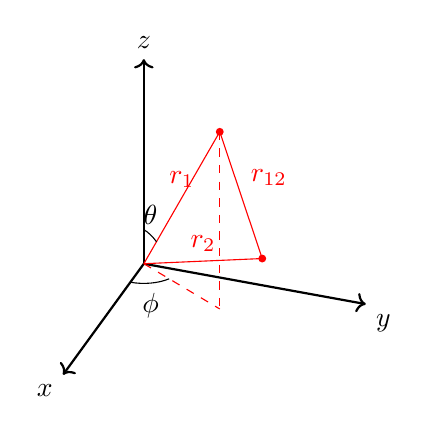
\begin{tikzpicture}[scale=1]

% Define parameters
\pgfmathsetmacro{\rvec}{3}
\pgfmathsetmacro{\thetavec}{30}
\pgfmathsetmacro{\phivec}{60}

\pgfmathsetmacro{\rtwovec}{10}
\pgfmathsetmacro{\thetatwovec}{60}
\pgfmathsetmacro{\phitwovec}{30}

% Set rotation angles for 3D visualization
\tdplotsetmaincoords{60}{110}

% Start drawing in 3D
\begin{scope}[tdplot_main_coords]

% Draw axes
\draw[thick,->] (0,0,0) -- (3,0,0) node[anchor=north east]{$x$};
\draw[thick,->] (0,0,0) -- (0,3,0) node[anchor=north west]{$y$};
\draw[thick,->] (0,0,0) -- (0,0,3) node[anchor=south]{$z$};

% Draw vector and its projections (with dashed lines)
\tdplotsetcoord{P}{\rvec}{\thetavec}{\phivec}
\draw[color=red] (0,0,0) -- (P) node[midway, above] {$r_1$};
\draw[dashed, color=red] (0,0,0) -- (Pxy);
\draw[dashed, color=red] (P) -- (Pxy);
\fill [red] (P) circle (0.05cm);

% Draw second electron
\tdplotsetcoord{P2}{\rtwovec}{\thetatwovec}{\phitwovec}
\draw[color=red] (0,0,0) -- (P2) node[midway, above] {$r_2$};
\fill [red] (P2) circle (0.05cm);

% Draw r12
\draw[color=red] (P) -- (P2) node[midway, above right] {$r_{12}$};

% Draw angle phi
\tdplotdrawarc{(0,0,0)}{0.5}{0}{\phivec}{anchor=north}{$\phi$}

% Draw angle theta
\tdplotsetthetaplanecoords{\phivec}
\tdplotdrawarc[tdplot_rotated_coords]{(0,0,0)}{0.5}{0}{\thetavec}{above}{$\theta$}

% this doesn't line up right
%\tdplotdrawarc[tdplot_rotated_coords]{(0,0,0)}{0.7}{\thetavec}{\thetatwovec}{anchor=south west}{$\psi$}

% this isn't the angle we need
%\tdplotdrawarc[tdplot_rotated_coords]{(0,0,0)}{0.7}{\thetavec}{66}{anchor=south west}{$\psi$}

\end{scope}
\end{tikzpicture}

% \begin{tikzpicture}
% \begin{axis}[
%     hide axis,
%     view={40}{-30},
%     samples=50
% ]
% \addplot3 [
%     surf,
% %    shader=interp,
%     domain=0:360,
%     y domain=-1:1,
%     fill opacity=0.1,
% ] (
%     {cos(x)*sqrt(1-y^2)},
%     {sin(x)*sqrt(1-y^2)},
%     y
% );
% 
% \addplot3 [
%     surf,
% %    shader=interp,
%     domain=0:360,
%     y domain=-1:1,
%     fill opacity=0.1,
% ] (
%     {0.5+cos(x)*sqrt(1-y^2)},
%     {0.5+sin(x)*sqrt(1-y^2)},
%     0.5+y
% );
% \end{axis}
% \end{tikzpicture}

\end{center}

\end{frame}

\begin{frame}
\frametitle{Helium Ground State Ansatz 16.6}
\begin{center}
\scalebox{0.9}{%
  \begin{tikzpicture}[remember picture,out=315,in=225,distance=0.4cm,node distance=40pt]
    \node (Psi) [poly, text width=100pt] {$\framebox(10,10){}\tikzmark{a}\,\Psi'' + \framebox(10,10){}\tikzmark{b}\,\Psi' + \coeff\tikzmark{c}\,\Psi$};
    \node (Qv) [ring, below of=Psi, text width=100pt] {$\mathbf{Q}[v]$};
    \node (v) [poly, right=of Qv] {$v$};
    \draw[degree] (a.west) -- (a.west|-Qv.north) node[right,pos=0.6] {2};
    \draw[degree] (b.west) -- (b.west|-Qv.north) node[right,pos=0.6] {2};
    \draw[degree] (c.west) -- (c.west|-Qv.north) node[right,pos=0.6] {2};
    \node (Psi label) [at=(v.east|-Psi.north), anchor=north east] {\Large$\Psi$};
    \begin{scope}[on background layer]
        \node (Psi block)[fit=(Psi) (Qv) (v), inner sep=10pt, element] {};
    \end{scope}
    \node (alg ext) [poly, node distance=150pt, below=of Psi.east, anchor=east, text width=100pt] {$\gamma^2 = \framebox(10,10){}\tikzmark{a}$};
    \begin{scope}[on background layer]
        \node (alg ext element) [algebraic, fit=(alg ext) (Psi label.east|-alg ext.north), inner sep=10pt] {};
        \node (alg ext title) [node distance=20pt, above=of alg ext element.north, anchor=center, text centered, text width=250pt] {$\mathbf{Q}[r_1,r_2,r_{12},\gamma]/(\gamma^2 - \coeff\,)$};
        \node (alg ext field) [ring, fill=none, fit=(alg ext title) (alg ext element), node distance=70pt, text width=250pt] {};
    \end{scope}
    \draw[degree] (v.south) -- (v.south|-alg ext field.north) node[right,pos=0.7] {2};
    \node (base) [ring, below=of alg ext field.south east, anchor=east, text width=250pt] {$\mathbf{Q}[r_1,r_2,r_{12}]$};
    \draw[degree] (a.west) -- (a.west|-base.north) node[right,pos=0.8] {2};
  \end{tikzpicture}
}
\end{center}
\end{frame}

\begin{frame}
\frametitle{Helium Ground State Ansatz 16.6}
\begin{center}
\bf
System of Polynomial Equations
\end{center}
\begin{itemize}
\item 33 variables
\item 3486 equations
\item 16,517,523 terms
\end{itemize}

\vskip 24pt

\begin{center}
\bf
Methods of Solving Systems of Polynomial Equations
\end{center}

\begin{itemize}
\item Primary Decomposition with Gr\"obner Bases
\item Numerical Optimization
\item Homotopy Continuation
\end{itemize}
\end{frame}

\lstset{
    basicstyle=\ttfamily,
    columns=fullflexible,
    keepspaces=true,
    showstringspaces=false,
    commentstyle=\color{gray},
    keywordstyle=\color{black},
    frame=none,
    framerule=0pt,
    aboveskip=0pt,
    belowskip=0pt,
    xleftmargin=0pt,
    xrightmargin=0pt,
    breaklines=true,
    breakatwhitespace=true,
    escapeinside={{*@}{@*}}
}

\begin{frame}[fragile]
\frametitle{Sage's {\tt primary_decomposition} doc string}
\tiny
\begin{adjustbox}{raise=10pt}
\begin{minipage}{\linewidth}
\begin{lstlisting}
*@\textcolor{blue}{sage:}@* ? I.primary_decomposition
*@\textcolor{red}{Call signature:}@*   I.primary_decomposition(*args, **kwds)
*@\textcolor{red}{Type:}@*            RequireField
*@\textcolor{red}{String form:}@*     <sage.rings.polynomial.multi_polynomial_ideal.RequireField object at 0x7fa439a00f70>
*@\textcolor{red}{File:}@*            /usr/lib/python3/dist-packages/sage/rings/polynomial/multi_polynomial_ideal.py
*@\textcolor{red}{Docstring:}@*
   Return a list of primary ideals such that their intersection is
   "self".

   An ideal Q is called primary if it is a proper ideal of the ring R,
   and if whenever ab in Q and a notin Q, then b^n in Q for some n
   in ZZ.

   If Q is a primary ideal of the ring R, then the radical ideal P of
   Q (i.e. the ideal consisting of all a in R with a^n in Q` for some
   n in ZZ), is called the associated prime of Q.

   If I is a proper ideal of a Noetherian ring R, then there exists a
   finite collection of primary ideals Q_i such that the following
   hold:

   * the intersection of the Q_i is I;

   * none of the Q_i contains the intersection of the others;

   * the associated prime ideals of the Q_i are pairwise distinct.

   INPUT:

   * "algorithm" -- string:

     * "'sy'" -- (default) use the Shimoyama-Yokoyama algorithm

     * "'gtz'" -- use the Gianni-Trager-Zacharias algorithm

   OUTPUT:

   * a list of primary ideals Q_i forming a primary decomposition of
     "self".


\end{lstlisting}
\end{minipage}
\end{adjustbox}
\end{frame}

\begin{frame}
%% \frametitle{Primary Decomposition with Gr\"obner Bases}
\frametitle{\tt https://www.singular.uni-kl.de/}

\includegraphics[page=1, clip, trim=0in 1in 0in 0in, width=\textwidth]{Singular Manual Singular Manual.pdf}
\end{frame}

\begin{frame}
\frametitle{Singular's Primary Decomposition Library}
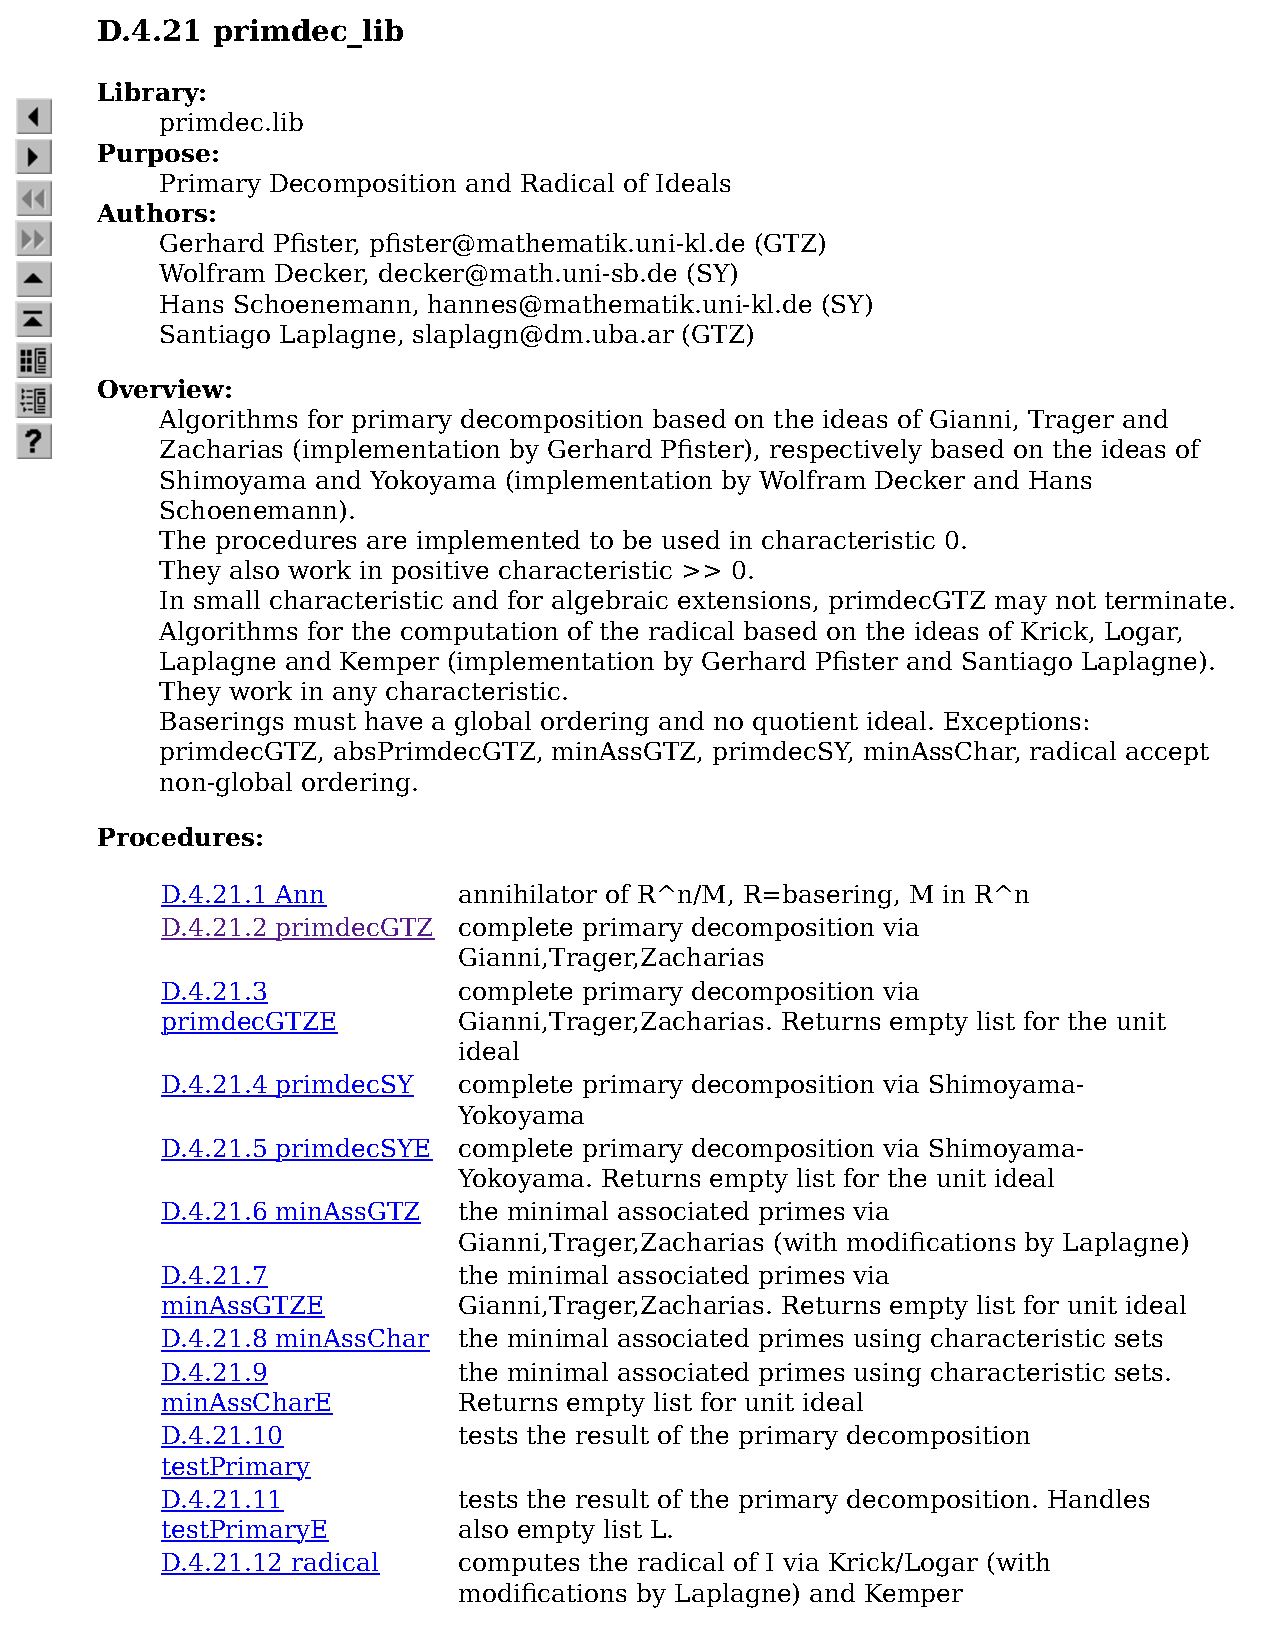
\includegraphics[page=1, clip, trim=0in 1in 0in 0in, width=\textwidth]{Singular Manual primdec_lib.pdf}
\end{frame}

\begin{frame}
\frametitle{Shimoyama and Yokoyama Algorithm}
% left bottom right top
\includegraphics[page=9, clip, trim=1.3in 4in 0in 5.1in, scale=0.9]{1-s2.0-S0747717196900528-main.pdf}

\vfill
\small
\begin{tabular}{ll}
Source: & Takeshi Shimoyama and Kazuhiro Yokoyama, \\
        & {\it Localization and Primary Decomposition of Polynomial Ideals}, \\
        & J. Symbolic Computation (1996) {\bf 22}, 247–277 \\
\end{tabular}
\end{frame}

\begin{frame}
\frametitle{Gr\"obner Bases}
\begin{definition}[Gr\"obner Basis]
Given a ring with a specified monomial order,
a {\it Gr\"obner Basis} or {\it standard basis} for an ideal $I$ is a set of
polynomials $G$ such that:
\begin{enumerate}
\item The polynomials in $G$ form a basis for the ideal $I$
\item The leading terms in $G$ form a basis for the ideal ${\rm lt}(I)$ formed by the leading terms in $I$.
\end{enumerate}
\end{definition}

\begin{example}
In the ring ${\mathbb Z}[x,y,z]$ with lexicographic ordering $x>y>z$, the ideal $(2x+3y+4z-5, 3x+4y+5z-2)$
has a reduced Gr\"obner basis given by
\begin{align*}
2x-2z+28 \\
3x-3z+42 \\
y+2z-11
\end{align*}
\end{example}
\end{frame}

\begin{frame}
\frametitle{Buchberger's Algorithm}

{\bf Input:} A set of polynomials $F$ that generates $I$

{\bf Output:} A Gröbner basis $G$ for $I$

\begin{enumerate}
\item $G := F$
\item For every $f_i,f_j$ in $G$, denote by $g_i$ the leading term of $f_i$ with respect to the given monomial ordering,
and by $a_{ij}$ the least common multiple of $g_i$ and $g_j$
\item Choose two polynomials in $G$ and let $S_{ij}=\frac{a_{ij}}{g_i}f_i  - \frac{a_{ij}}{g_j}f_j $

(Note that the leading terms here will cancel by construction).
\item Reduce $S_{ij}$, with the multivariate division algorithm relative to the set $G$ until the result is not further reducible.

If the result is non-zero, add it to $G$.
\item Repeat steps 2-4 until all possible pairs are considered, including those involving the new polynomials added in step 4.
\item Output $G$
\end{enumerate}

Source: Wikipedia, {\it Buchberger's Algorithm}
\end{frame}

\begin{frame}
\frametitle{Desired features of a Gr\"obner basis algorithm}
\begin{itemize}
\item Selection of s-pairs guided by a machine learning algorithm
\item Modular: operate modulo primes and lift results back to $\mathbb Z$
\item Fall back on disk efficiently when RAM exhausted
\end{itemize}
\end{frame}

\begin{frame}
\frametitle{Disk based Gr\"obner basis algorithm}

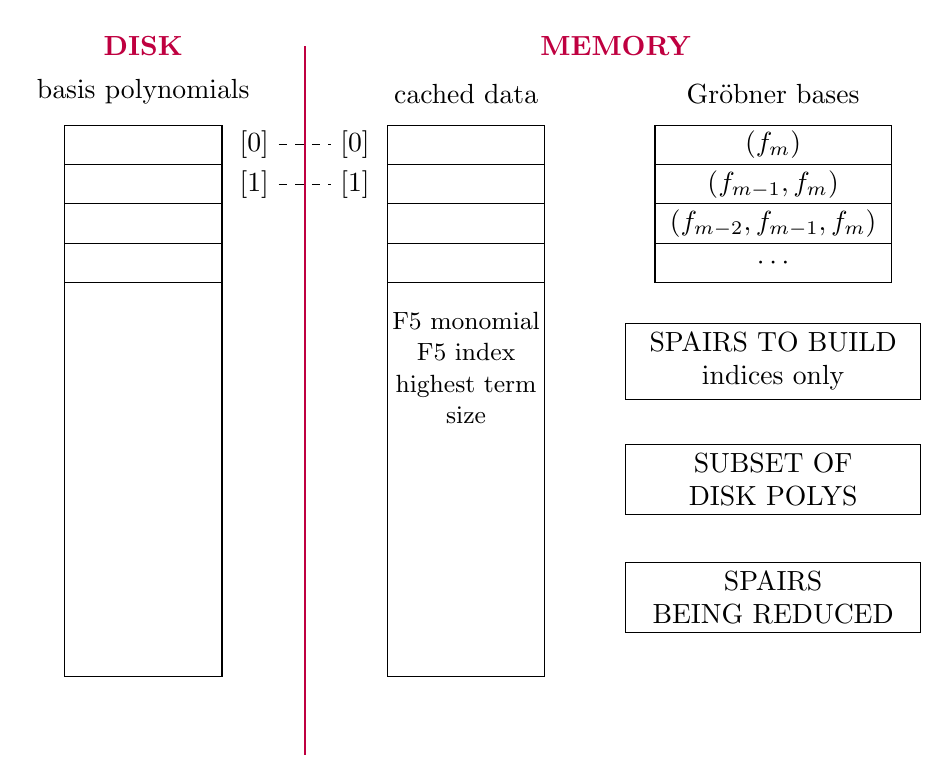
\begin{tikzpicture}
  % Define the dimensions of the array
  \def\numRows{3}
  \def\sliceHeight{0.5}
  \def\sliceWidth{2}
  \def\labelOffset{0.1}

  % Draw the array (the disk copy)
  \foreach \j in {0,...,\numRows} {
    \draw (0,\j*\sliceHeight) rectangle (\sliceWidth,\j*\sliceHeight+\sliceHeight);
  }
  \node[right] (disk0) at (\sliceWidth+\labelOffset,3*\sliceHeight+0.5*\sliceHeight) {[0]};
  \node[right] (disk1) at (\sliceWidth+\labelOffset,2*\sliceHeight+0.5*\sliceHeight) {[1]};

  \node[above=0.4, align=center] at (\sliceWidth/2,3*\sliceHeight+0.5*\sliceHeight) {basis polynomials};

  \draw (0,-10*\sliceHeight) rectangle (\sliceWidth,0);

% another array (the in-memory copy)
\begin{scope}[xshift=4.1cm]
  \foreach \j in {0,...,\numRows} {
    \draw (0,\j*\sliceHeight) rectangle (\sliceWidth,\j*\sliceHeight+\sliceHeight);
  }
  \node[left] (mem0) at (-\labelOffset,3*\sliceHeight+0.5*\sliceHeight) {[0]};
  \node[left] (mem1) at (-\labelOffset,2*\sliceHeight+0.5*\sliceHeight) {[1]};

  \node[above=0.4, align=center] at (\sliceWidth/2,3*\sliceHeight+0.5*\sliceHeight) {cached data};

  \node[below=2, align=center] at (\sliceWidth/2,3*\sliceHeight+0.5*\sliceHeight) {\small F5 monomial};
  \node[below=2.4, align=center] at (\sliceWidth/2,3*\sliceHeight+0.5*\sliceHeight) {\small F5 index};
  \node[below=2.8, align=center] at (\sliceWidth/2,3*\sliceHeight+0.5*\sliceHeight) {\small highest term};
  \node[below=3.2, align=center] at (\sliceWidth/2,3*\sliceHeight+0.5*\sliceHeight) {\small size};


  \draw (0,-10*\sliceHeight) rectangle (\sliceWidth,0);
\end{scope}

% another array (the older Grobner bases)
  \def\sliceWidth{3}
\begin{scope}[xshift=7.5cm]
  \draw (0,0*\sliceHeight) rectangle (\sliceWidth,0*\sliceHeight+\sliceHeight) node [midway] {$\cdots$};
  \draw (0,1*\sliceHeight) rectangle (\sliceWidth,1*\sliceHeight+\sliceHeight) node [midway] {$(f_{m-2}, f_{m-1}, f_m)$};
  \draw (0,2*\sliceHeight) rectangle (\sliceWidth,2*\sliceHeight+\sliceHeight) node [midway] {$(f_{m-1}, f_m)$};
  \draw (0,3*\sliceHeight) rectangle (\sliceWidth,3*\sliceHeight+\sliceHeight) node [midway] {$(f_m)$} node [midway, above=0.4] {Gr\"obner bases};
%  \node[left] (mem0) at (-\labelOffset,3*\sliceHeight+0.5*\sliceHeight) {[0]};
%  \node[left] (mem1) at (-\labelOffset,2*\sliceHeight+0.5*\sliceHeight) {[1]};
\end{scope}

  % dashed lines between the disk and the memory
  \draw [dashed] (disk0.east) -- (mem0.west);
  \draw [dashed] (disk1.east) -- (mem1.west);

  % lines dividing disk from memory
  \draw [purple,thick] (3.05cm,3) -- (3.05cm,-6);
  \node [purple,align=center] at (1,3) {\bf DISK};
  \node [purple,align=center] at (7,3) {\bf MEMORY};

  \node [draw, align=center, text width=100pt] at (9,-1) {SPAIRS TO BUILD\break indices only};

  \node [draw, align=center, text width=100pt] at (9,-2.5) {SUBSET OF DISK POLYS};

  \node [draw, align=center, text width=100pt] at (9,-4) {SPAIRS\break BEING REDUCED};


\end{tikzpicture}

\end{frame}

\begin{frame}[fragile]
\frametitle{Use of Large Language Models in Software Development}
\scriptsize
\begin{verbatim}
include(common)

Function buchberger_naive maintains two local vectors of polynomials,
 called the basis and the s-pairs.  Start by copying the vector of
 generators to the basis.  For each pair of generators, construct their
 s-pair and insert it into the s-pairs if it is unique.  Then work through
 the vector of s-pairs from beginning to end, reducing each one by the
 basis.  Use reduce_by_vector with lead reduction enabled.  If the result
 is not zero, then append the result to the basis, and loop over all of the
 other basis polynomials, constructing the s-pair of it and the new basis
 polynomial, and appending it to the s-pairs if it is unique.  Make sure to
 process all of the s-pairs, even the ones added during processing.

Function buchberger_naive puts the basis in the output vector
once the loop has terminated, and returns void.

You can not add items to a polynomial vector by calling fmpz_mpoly_set
 with an fmpz_mpoly_vec_entry as your destination; you have to use
 fmpz_mpoly_vec_append.

Output the header, any required function declarations, the code for
 buchberger_naive, and nothing else, without any explaination.

Output no function defintions except the code for buchberger_naive.
\end{verbatim}
\end{frame}

\begin{frame}
\frametitle{Numerical Optimization}
\begin{itemize}
\item Use numerical root-finding techniques (gradient descent, Levenburg-Marquardt, {\tt scipy}) to find an approximate zero
\item We get a {\it witness point}: an approximate solution good enough to recover the exact solution ({\it exactness recovery})
\item Ex: 1.0000057 is approximately 1
\item This works well for finding a single prime component
\item The problem is how to remove a prime component so you can find all the prime components
\item The best way I've found to remove prime components is to use the {\it Euclidean Distance} function
to drive solutions away from known components by introducing an extra function whose value becomes large
as you approach a known solution
\end{itemize}
\end{frame}

\begin{frame}
\frametitle{The Euclidean Distance Function}

\includegraphics[page=3, clip, trim=0in 1in 0in 0in, width=\textwidth]{The_distance_function_from_a_real_algebraic_variety_]_Giorgio_Ottaviani,_University_of_Florence.pdf}
\begin{block}{}
Source: Giorgio Ottaviani, {\it The distance function from an algebraic variety}, {\it Nonlinear Algebra in Applications}, ICERM workshop, 2018
\end{block}
\end{frame}

\begin{frame}
\frametitle{The Euclidean Distance Function}

\includegraphics[page=7, clip, trim=0in 0in 0in 0in, width=\textwidth]{The_distance_function_from_a_real_algebraic_variety_]_Giorgio_Ottaviani,_University_of_Florence.pdf}
\end{frame}

\begin{frame}
\frametitle{The Euclidean Distance Function}

\includegraphics[page=15, clip, trim=0in 0in 0in 0in, width=\textwidth]{The_distance_function_from_a_real_algebraic_variety_]_Giorgio_Ottaviani,_University_of_Florence.pdf}
\end{frame}

\begin{frame}
\frametitle{Euclidean Distance polynomial for the ellipse $4x^2 + y^2 = 1$}
\scriptsize
\[ 144 \, t^{8} - 24 \, {\left(28 \, x^{2} + 8 \, y^{2} + 15\right)} t^{6} \]
\[ + {\left(1168 \, x^{4} + 992 \, x^{2} y^{2} - 32 \, y^{4} + 1080 \, x^{2} - 360 \, y^{2} + 297\right)} t^{4} \]
\[ - 2 \, {\left(448 \, x^{6} + 720 \, x^{4} y^{2} + 240 \, x^{2} y^{4} - 32 \, y^{6} + 496 \, x^{4} - 280 \, x^{2} y^{2} + 124 \, y^{4} + 180 \, x^{2} - 135 \, y^{2} + 45\right)} t^{2} \]
\[ + 256 \, x^{6} - 480 \, x^{4} y^{2} - 360 \, x^{2} y^{4} - 56 \, y^{6} + 256 \, x^{8} + 640 \, x^{6} y^{2} + 528 \, x^{4} y^{4} + 160 \, x^{2} y^{6} + 16 \, y^{8} \]
\[ - 32 \, x^{4} + 248 \, x^{2} y^{2} + 73 \, y^{4} - 48 \, x^{2} - 42 \, y^{2} + 9 = 0 \]
\end{frame}

\begin{frame}[fragile]
\frametitle{Euclidean Distance from $(1,1)$ to the ellipse $4x^2 + y^2 = 1$}
To find the distance from the point $(1,1)$ to the ellipse $4x^2 + y^2 = 1$, we substitute $x=1$ and $y=1$ into
the Euclidean Distance polynomial:

\[ 144 t^{8} - 1224 t^{6} + 3145 t^{4} - 3612 t^{2} + 1168 \]

We want the smallest positive real root of this polynomial

\begin{verbatim}
sage: [N(sol[0]) for sol in SRbwb.roots()]                                                                                         
[-2.26742176878493,
 2.26742176878493,
 -0.709400520758237,
 0.709400520758237,
 -1.26458649349997 - 0.414010009237062*I,
 1.26458649349997 + 0.414010009237062*I,
 -1.26458649349997 + 0.414010009237062*I,
 1.26458649349997 - 0.414010009237062*I]
\end{verbatim}
\end{frame}

\begin{frame}[fragile]
\frametitle{Euclidean Distance from $(1,1)$ to the ellipse $4x^2 + y^2 = 1$}
\begin{center}
\makebox[.3\linewidth][l]{
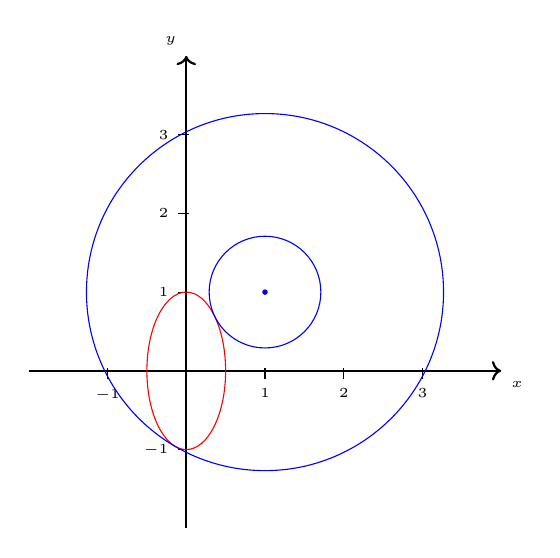
\begin{tikzpicture}[baseline={(0,1.6)}]
    % Draw axes
    \draw[thick,->] (-2,0) -- (4,0) node[anchor=north west, font=\tiny] {$x$};
    \draw[thick,->] (0,-2) -- (0,4) node[anchor=south east, font=\tiny] {$y$};

    % Draw grid with labels
    \foreach \x in {-1,1,2,3} {
        \draw (\x,1pt) -- (\x,-3pt) node[anchor=north, font=\tiny] {$\x$};
        \draw (1pt,\x) -- (-3pt,\x) node[anchor=east, font=\tiny] {$\x$};
    }

    \draw [red] (0,0) ellipse (0.5 and 1);
    \fill [blue] (1,1) circle (1pt);
    \draw [blue] (1,1) circle (0.7094);
    \draw [blue] (1,1) circle (2.2674);
\end{tikzpicture}
}%
\begin{minipage}[b]{.8\linewidth}
\tiny
\begin{verbatim}
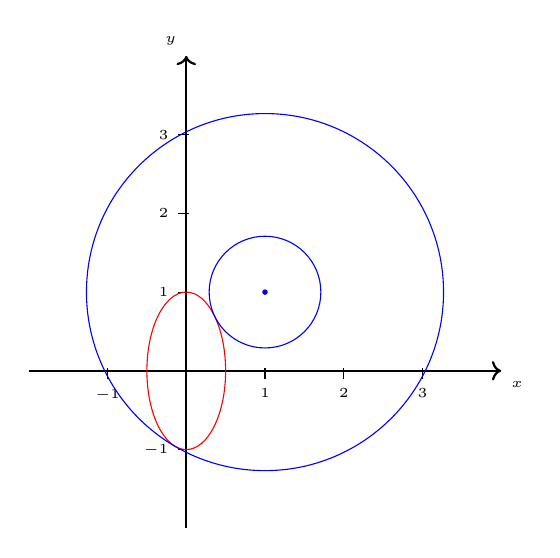
\begin{tikzpicture}
    % Draw axes
    \draw[thick,->] (-2,0) -- (4,0) node[anchor=north west, font=\tiny] {$x$};
    \draw[thick,->] (0,-2) -- (0,4) node[anchor=south east, font=\tiny] {$y$};

    % Draw grid with labels
    \foreach \x in {-1,1,2,3} {
        \draw (\x,1pt) -- (\x,-3pt) node[anchor=north, font=\tiny] {$\x$};
        \draw (1pt,\x) -- (-3pt,\x) node[anchor=east, font=\tiny] {$\x$};
    }

    \draw [red] (0,0) ellipse (0.5 and 1);
    \fill [blue] (1,1) circle (1pt);
    \draw [blue] (1,1) circle (0.7094);
    \draw [blue] (1,1) circle (2.2674);
\end{tikzpicture}
\end{verbatim}
\end{minipage}
\end{center}
\end{frame}

\begin{frame}
\frametitle{The Euclidean Distance Function}

\includegraphics[page=16, clip, trim=0in 0in 0in 0in, width=\textwidth]{The_distance_function_from_a_real_algebraic_variety_]_Giorgio_Ottaviani,_University_of_Florence.pdf}
Source: Ottaviani, {\it The distance function from an algebraic variety}, {\it Nonlinear Algebra in Applications}, ICERM workshop, 2018
\end{frame}

\begin{frame}[fragile]
\frametitle{Computing EDpoly$_{4x^2+y^2-1}$ using Sage}
\scriptsize
\begin{verbatim}
import itertools

RED.<x,y,ux,uy,t> = PolynomialRing(QQ, 5, order='degrevlex(2), degrevlex(3)')
I=ideal(4*x^2 + y^2 - 1)
Jacobian = matrix([[g.derivative(RED(cv)) for g in I.gens()] for cv in [x,y]])
extendedJacobian = Jacobian.transpose().stack(matrix([RED('u' + str(cv)) - RED(cv)
    for cv in [x,y]]))
\end{verbatim}
\[
\left(\begin{array}{rr}
8 x & 2 y \\
-x + \mathit{ux} & -y + \mathit{uy}
\end{array}\right)
\]
\begin{verbatim}
minors = [extendedJacobian.determinant()]
critical_ideal_generators = [g for g in itertools.chain(minors, I.gens())]
distance_function = t^2 - sum((RED(cv) - RED('u'+str(cv)))^2 for cv in [x,y])
elimination_ideal = ideal(critical_ideal_generators + [distance_function])
GB = elimination_ideal.groebner_basis()
GB[-1].numerator()
GB[-1].numerator().subs(ux=1,uy=1)
\end{verbatim}
\end{frame}

\begin{frame}[fragile]
\frametitle{Bertini - {\tt bertini.nd.edu}}
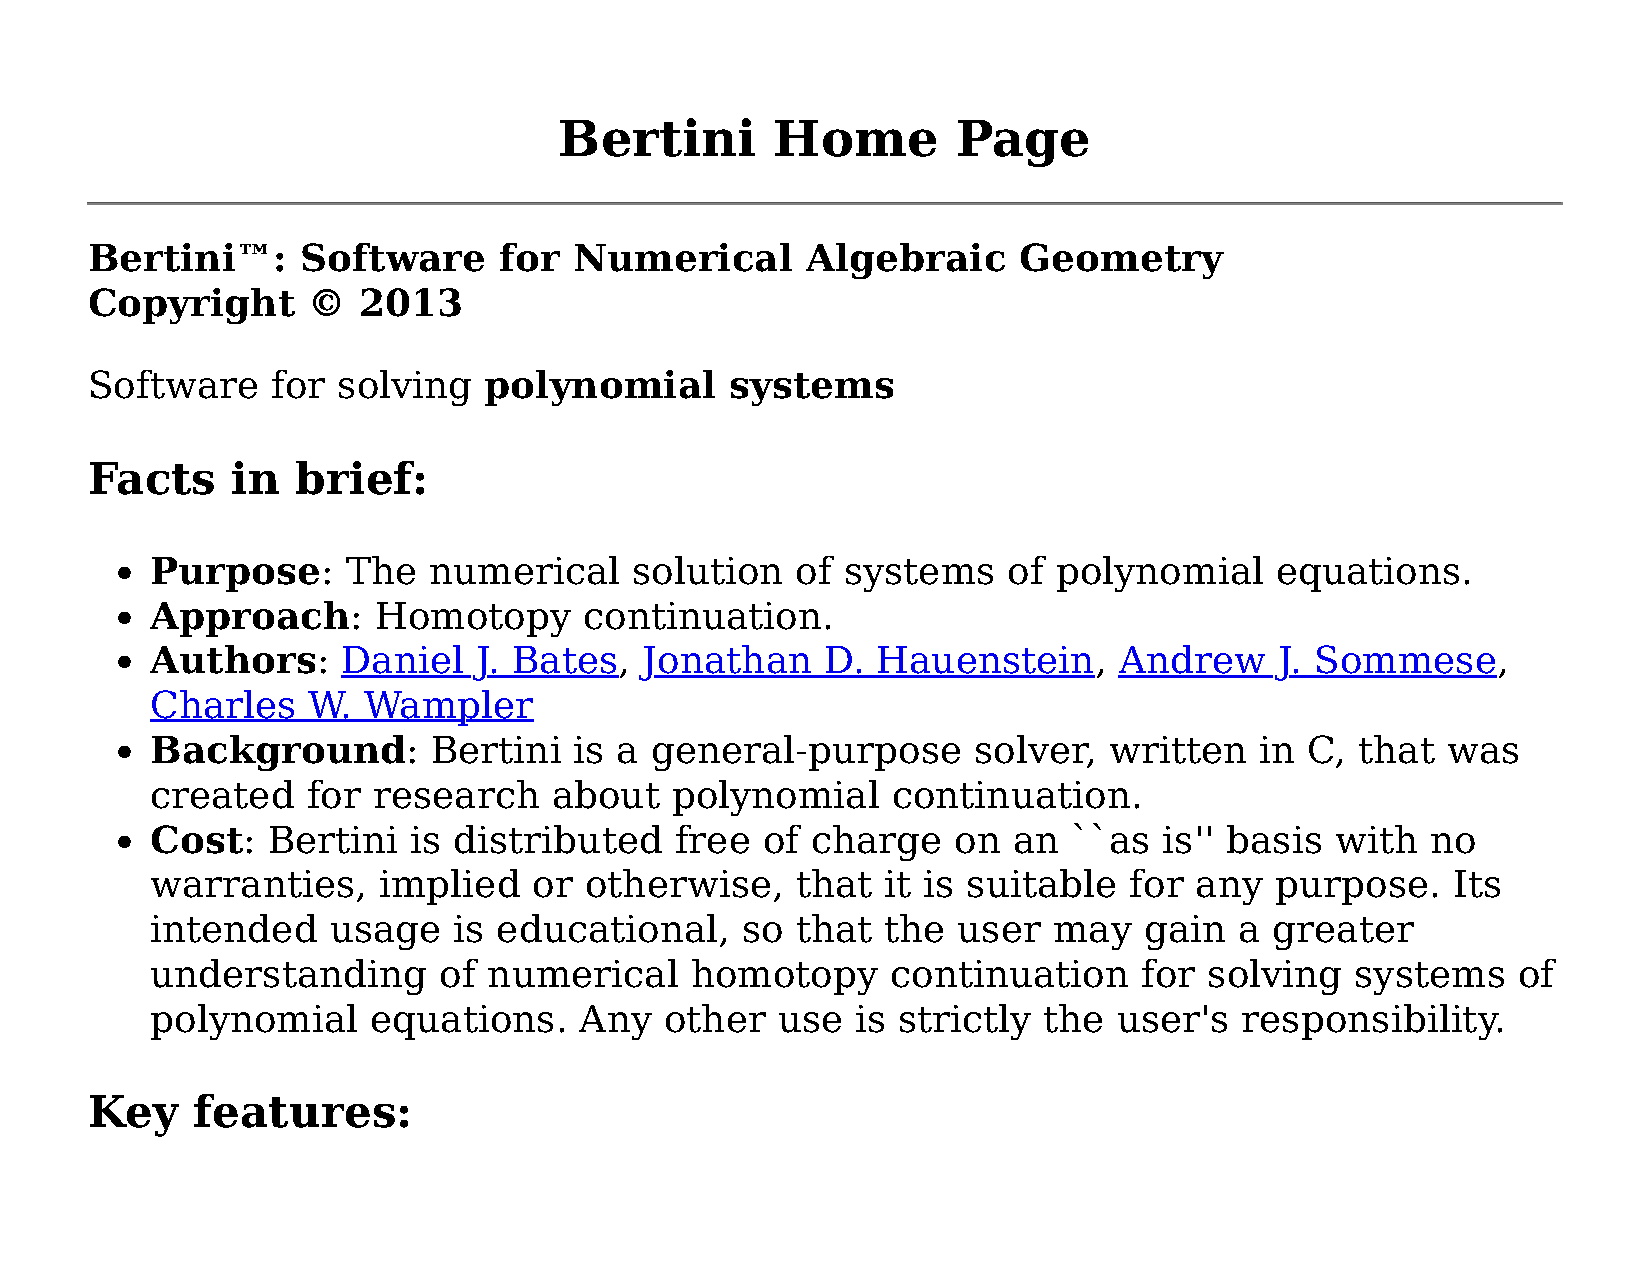
\includegraphics[page=1, clip, trim=0in 1.5in 0in 0in, width=\textwidth]{bertini.nd.edu.pdf}
\end{frame}

\begin{frame}
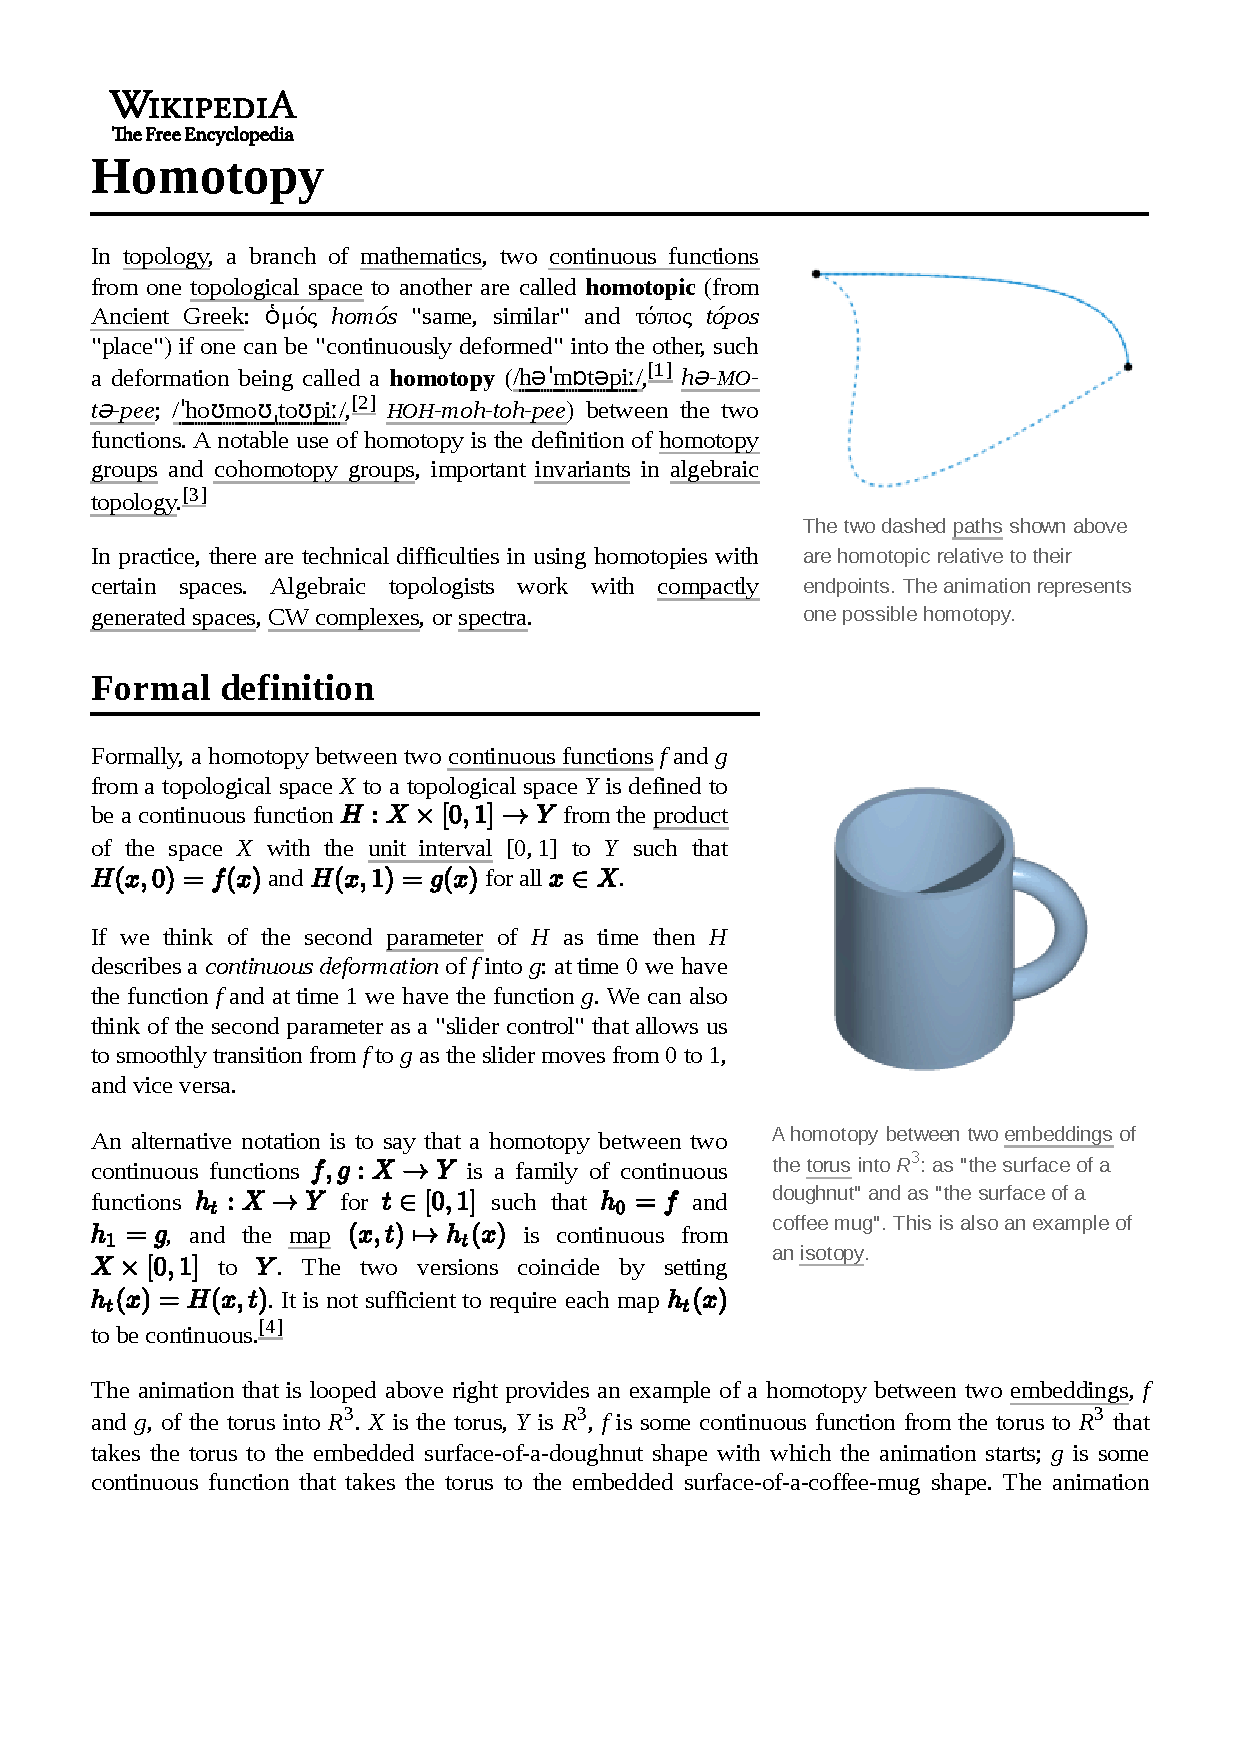
\includegraphics[width=\textwidth]{Homotopy.pdf}
\end{frame}

\begin{frame}
\frametitle{Homotopy Continuation}
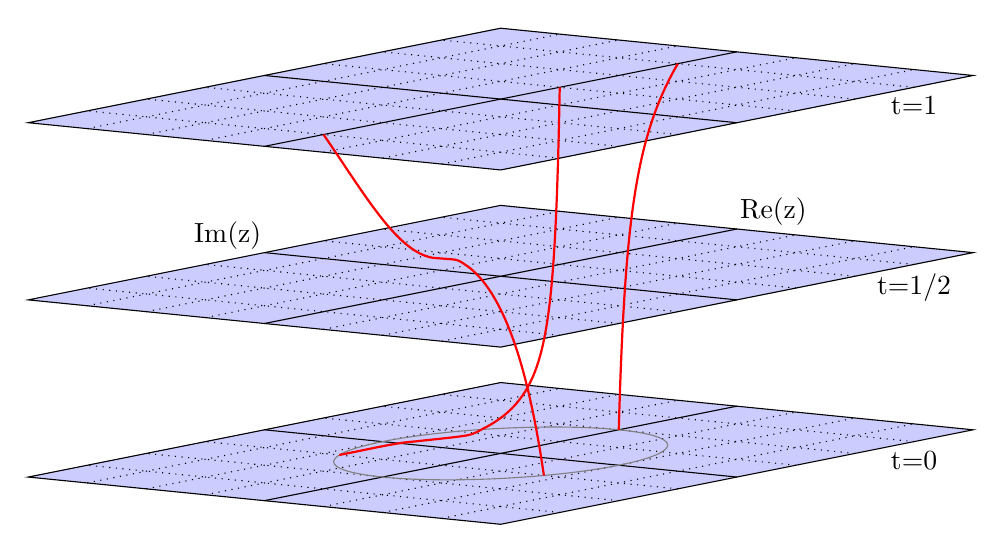
\begin{tikzpicture}[scale=1.5, x={(1cm,0.2cm)}, y={(-1cm,0.1cm)}, z={(0cm,0.75cm)}]

  % the three coordinate planes
  \foreach \z in {0,2,4} {
     \draw[fill=blue!20] (-2,-2,\z) -- (2,-2,\z) -- (2,2,\z) -- (-2,2,\z) -- cycle;
     \draw (2,0,\z) -- (-2,0,\z);
     \draw (0,2,\z) -- (0,-2,\z);
     \foreach \x in {-1.5,-1,-0.5,0.5,1,1.5} {
        \draw [dotted] (\x,-2,\z) -- (\x,2,\z);
        \draw [dotted] (-2,\x,\z) -- (2,\x,\z);
     }
  }

  % Draw the axes labels
  \node[inner sep=1pt, above right] at (2,0,2) {Re(z)};
  \node[inner sep=1pt, above left] at (0,2,2) {Im(z)};

  % Draw the t labels
  \node[below] at (1.5,-2,0) {t=0};
  \node[below] at (1.5,-2,2) {t=1/2};
  \node[below] at (1.5,-2,4) {t=1};

  \draw [gray] (0,0,0) circle (1);

  \draw[red, thick, smooth] plot coordinates {
( -0.500000000000000 , 0.866025403784439 , 0.000000000000000 )
( -0.489633209316899 , 0.766554518836523 , 0.0400000000000000 )
( -0.481511768921815 , 0.668843685993489 , 0.0800000000000000 )
( -0.475190957404572 , 0.570430625180296 , 0.120000000000000 )
( -0.470318531771919 , 0.467630406333101 , 0.160000000000000 )
( -0.466612987397390 , 0.353230906528125 , 0.200000000000000 )
( -0.463847991950720 , 0.204193991215259 , 0.240000000000000 )
( -0.282484157335666 , 0.000000000000000 , 0.280000000000000 )
( -0.147152860688391 , -1.11022302462516e-16 , 0.320000000000000 )
( -0.0628562467541067 , 0.000000000000000 , 0.360000000000000 )
( 0.000000000000000 , 0 , 0.400000000000000 )
( 0.0500603013171183 , 0.000000000000000 , 0.440000000000000 )
( 0.0913868437398897 , 0.000000000000000 , 0.480000000000000 )
( 0.126304703982792 , 1.11022302462516e-16 , 0.520000000000000 )
( 0.156301461790679 , 0.000000000000000 , 0.560000000000000 )
( 0.182399400450203 , 0.000000000000000 , 0.600000000000000 )
( 0.205336730296717 , -1.11022302462516e-16 , 0.640000000000000 )
( 0.225666192336757 , 0.000000000000000 , 0.680000000000000 )
( 0.243813233843055 , 0.000000000000000 , 0.720000000000000 )
( 0.260112512666214 , -1.11022302462516e-16 , 0.760000000000000 )
( 0.274831936294719 , 2.22044604925031e-16 , 0.800000000000000 )
( 0.288189116907647 , 1.11022302462516e-16 , 0.840000000000000 )
( 0.300362996524422 , 0.000000000000000 , 0.880000000000000 )
( 0.311502277722306 , 1.11022302462516e-16 , 0.920000000000000 )
( 0.321731673586785 , -2.22044604925031e-16 , 0.960000000000000 )
( 0.331156628382010 , -1.11022302462516e-16 , 1.00000000000000 )
( 0.339866940873570 , -2.22044604925031e-16 , 1.04000000000000 )
( 0.347939584464723 , -1.11022302462516e-16 , 1.08000000000000 )
( 0.355440929215222 , 1.11022302462516e-16 , 1.12000000000000 )
( 0.362428511657882 , -1.11022302462516e-16 , 1.16000000000000 )
( 0.368952458126070 , 0.000000000000000 , 1.20000000000000 )
( 0.375056639412920 , 1.11022302462516e-16 , 1.24000000000000 )
( 0.380779614871294 , -1.11022302462516e-16 , 1.28000000000000 )
( 0.386155409901620 , 1.11022302462516e-16 , 1.32000000000000 )
( 0.391214160448139 , 1.11022302462516e-16 , 1.36000000000000 )
( 0.395982650492782 , -2.22044604925031e-16 , 1.40000000000000 )
( 0.400484762827656 , -1.11022302462516e-16 , 1.44000000000000 )
( 0.404741859069956 , 0.000000000000000 , 1.48000000000000 )
( 0.408773101585006 , 0.000000000000000 , 1.52000000000000 )
( 0.412595727440196 , 0.000000000000000 , 1.56000000000000 )
( 0.416225282535081 , 2.22044604925031e-16 , 1.60000000000000 )
( 0.419675822503145 , -2.22044604925031e-16 , 1.64000000000000 )
( 0.422960085757134 , 0.000000000000000 , 1.68000000000000 )
( 0.426089643077437 , 0.000000000000000 , 1.72000000000000 )
( 0.429075027365091 , 0.000000000000000 , 1.76000000000000 )
( 0.431925846555173 , 0.000000000000000 , 1.80000000000000 )
( 0.434650882179950 , 0.000000000000000 , 1.84000000000000 )
( 0.437258175659387 , -1.11022302462516e-16 , 1.88000000000000 )
( 0.439755104060005 , -1.11022302462516e-16 , 1.92000000000000 )
( 0.442148446786728 , 2.22044604925031e-16 , 1.96000000000000 )
( 0.444444444444444 , 0 , 2.00000000000000 )
( 0.446648850917221 , 0.000000000000000 , 2.04000000000000 )
( 0.448766979556164 , -2.22044604925031e-16 , 2.08000000000000 )
( 0.450803744235908 , -1.11022302462516e-16 , 2.12000000000000 )
( 0.452763695929975 , 2.22044604925031e-16 , 2.16000000000000 )
( 0.454651055363002 , 2.22044604925031e-16 , 2.20000000000000 )
( 0.456469742220038 , 0.000000000000000 , 2.24000000000000 )
( 0.458223401327278 , 1.11022302462516e-16 , 2.28000000000000 )
( 0.459915426162758 , 0.000000000000000 , 2.32000000000000 )
( 0.461548980007981 , 2.22044604925031e-16 , 2.36000000000000 )
( 0.463127015010862 , 0.000000000000000 , 2.40000000000000 )
( 0.464652289395670 , 0.000000000000000 , 2.44000000000000 )
( 0.466127383025794 , 0.000000000000000 , 2.48000000000000 )
( 0.467554711499588 , 0.000000000000000 , 2.52000000000000 )
( 0.468936538937372 , 1.11022302462516e-16 , 2.56000000000000 )
( 0.470274989598616 , -1.11022302462516e-16 , 2.60000000000000 )
( 0.471572058451711 , 0.000000000000000 , 2.64000000000000 )
( 0.472829620804421 , 2.22044604925031e-16 , 2.68000000000000 )
( 0.474049441090540 , 2.22044604925031e-16 , 2.72000000000000 )
( 0.475233180897404 , -2.22044604925031e-16 , 2.76000000000000 )
( 0.476382406309365 , 0.000000000000000 , 2.80000000000000 )
( 0.477498594633992 , 3.33066907387547e-16 , 2.84000000000000 )
( 0.478583140570437 , 1.11022302462516e-16 , 2.88000000000000 )
( 0.479637361872994 , 0.000000000000000 , 2.92000000000000 )
( 0.480662504557188 , 0.000000000000000 , 2.96000000000000 )
( 0.481659747690771 , -1.11022302462516e-16 , 3.00000000000000 )
( 0.482630207807565 , 0.000000000000000 , 3.04000000000000 )
( 0.483574942978214 , 0.000000000000000 , 3.08000000000000 )
( 0.484494956568431 , -1.11022302462516e-16 , 3.12000000000000 )
( 0.485391200712277 , 0.000000000000000 , 3.16000000000000 )
( 0.486264579525253 , 0.000000000000000 , 3.20000000000000 )
( 0.487115952079604 , -1.11022302462516e-16 , 3.24000000000000 )
( 0.487946135162012 , 2.22044604925031e-16 , 3.28000000000000 )
( 0.488755905831970 , 0.000000000000000 , 3.32000000000000 )
( 0.489546003797386 , 0.000000000000000 , 3.36000000000000 )
( 0.490317133622405 , 0.000000000000000 , 3.40000000000000 )
( 0.491069966781070 , 0.000000000000000 , 3.44000000000000 )
( 0.491805143569193 , 0.000000000000000 , 3.48000000000000 )
( 0.492523274885690 , -1.11022302462516e-16 , 3.52000000000000 )
( 0.493224943893615 , -1.11022302462516e-16 , 3.56000000000000 )
( 0.493910707570251 , 0.000000000000000 , 3.60000000000000 )
( 0.494581098154761 , -1.11022302462516e-16 , 3.64000000000000 )
( 0.495236624501199 , -2.22044604925031e-16 , 3.68000000000000 )
( 0.495877773343995 , 0.000000000000000 , 3.72000000000000 )
( 0.496505010482421 , -1.11022302462516e-16 , 3.76000000000000 )
( 0.497118781890018 , -2.22044604925031e-16 , 3.80000000000000 )
( 0.497719514754447 , -1.11022302462516e-16 , 3.84000000000000 )
( 0.498307618452789 , 0.000000000000000 , 3.88000000000000 )
( 0.498883485466904 , 0.000000000000000 , 3.92000000000000 )
( 0.499447492243100 , 0.000000000000000 , 3.96000000000000 )
( 0.500000000000000 , 0 , 4.00000000000000 )
};

  \draw[red, thick, smooth] plot coordinates {
( -0.500000000000000 , -0.866025403784439 , 0.000000000000000 )
( -0.499414625636490 , -0.860929901761194 , 0.0400000000000000 )
( -0.498825172684574 , -0.855745350822177 , 0.0800000000000000 )
( -0.498231648524139 , -0.850469158096479 , 0.120000000000000 )
( -0.497634063595094 , -0.845098617510188 , 0.160000000000000 )
( -0.497032431613426 , -0.839630902851258 , 0.200000000000000 )
( -0.496426769801168 , -0.834063060270287 , 0.240000000000000 )
( -0.495817099131194 , -0.828392000159103 , 0.280000000000000 )
( -0.495203444587832 , -0.822614488341803 , 0.320000000000000 )
( -0.494585835444316 , -0.816727136504484 , 0.360000000000000 )
( -0.493964305558214 , -0.810726391780290 , 0.400000000000000 )
( -0.493338893686011 , -0.804608525395259 , 0.440000000000000 )
( -0.492709643818131 , -0.798369620267542 , 0.480000000000000 )
( -0.492076605535738 , -0.792005557437622 , 0.520000000000000 )
( -0.491439834390800 , -0.785512001189656 , 0.560000000000000 )
( -0.490799392310936 , -0.778884382703706 , 0.600000000000000 )
( -0.490155348030726 , -0.772117882054634 , 0.640000000000000 )
( -0.489507777551239 , -0.765207408345296 , 0.680000000000000 )
( -0.488856764629677 , -0.758147577728334 , 0.720000000000000 )
( -0.488202401301154 , -0.750932689031391 , 0.760000000000000 )
( -0.487544788434753 , -0.743556696653508 , 0.800000000000000 )
( -0.486884036326169 , -0.736013180344223 , 0.840000000000000 )
( -0.486220265329388 , -0.728295311409280 , 0.880000000000000 )
( -0.485553606530000 , -0.720395814805302 , 0.920000000000000 )
( -0.484884202462960 , -0.712306926486826 , 0.960000000000000 )
( -0.484212207877737 , -0.704020345248501 , 1.00000000000000 )
( -0.483537790554026 , -0.695527178157378 , 1.04000000000000 )
( -0.482861132171387 , -0.686817878487953 , 1.08000000000000 )
( -0.482182429236373 , -0.677882174846550 , 1.12000000000000 )
( -0.481501894070961 , -0.668708989889328 , 1.16000000000000 )
( -0.480819755866319 , -0.659286346683486 , 1.20000000000000 )
( -0.480136261806169 , -0.649601260311966 , 1.24000000000000 )
( -0.479451678264298 , -0.639639611748815 , 1.28000000000000 )
( -0.478766292080998 , -0.629386000294857 , 1.32000000000000 )
( -0.478080411923499 , -0.618823569905998 , 1.36000000000000 )
( -0.477394369735730 , -0.607933803491921 , 1.40000000000000 )
( -0.476708522283038 , -0.596696277601779 , 1.44000000000000 )
( -0.476023252797747 , -0.585088367689740 , 1.48000000000000 )
( -0.475338972731756 , -0.573084891140205 , 1.52000000000000 )
( -0.474656123622622 , -0.560657671096879 , 1.56000000000000 )
( -0.473975179079859 , -0.547774998381979 , 1.60000000000000 )
( -0.473296646898419 , -0.534400960650140 , 1.64000000000000 )
( -0.472621071306574 , -0.520494596210574 , 1.68000000000000 )
( -0.471949035355598 , -0.506008812785137 , 1.72000000000000 )
( -0.471281163458815 , -0.490888985774964 , 1.76000000000000 )
( -0.470618124087693 , -0.475071111233913 , 1.80000000000000 )
( -0.469960632632713 , -0.458479326796327 , 1.84000000000000 )
( -0.469309454436696 , -0.441022513370413 , 1.88000000000000 )
( -0.468665408008149 , -0.422589521894477 , 1.92000000000000 )
( -0.468029368421954 , -0.403042275260425 , 1.96000000000000 )
( -0.467402270914302 , -0.382205457425598 , 2.00000000000000 )
( -0.466785114678234 , -0.359850461485394 , 2.04000000000000 )
( -0.466178966865390 , -0.335669117577676 , 2.08000000000000 )
( -0.465584966798540 , -0.309227886715316 , 2.12000000000000 )
( -0.465004330398217 , -0.279881110400506 , 2.16000000000000 )
( -0.464438354825164 , -0.246586967436159 , 2.20000000000000 )
( -0.463888423338329 , -0.207445760395285 , 2.24000000000000 )
( -0.463356010365769 , -0.158164752156479 , 2.28000000000000 )
( -0.462842686782922 , -0.0821526077997757 , 2.32000000000000 )
( -0.570841661752826 , 0.000000000000000 , 2.36000000000000 )
( -0.636652133789091 , 0.000000000000000 , 2.40000000000000 )
( -0.684096489281377 , -1.11022302462516e-16 , 2.44000000000000 )
( -0.723450955576166 , 1.66533453693773e-16 , 2.48000000000000 )
( -0.757996839083920 , 1.11022302462516e-16 , 2.52000000000000 )
( -0.789284693625066 , 0.000000000000000 , 2.56000000000000 )
( -0.818192830826646 , -5.55111512312578e-17 , 2.60000000000000 )
( -0.845275756709078 , -5.55111512312578e-17 , 2.64000000000000 )
( -0.870910087754895 , 1.11022302462516e-16 , 2.68000000000000 )
( -0.895365523104081 , 0.000000000000000 , 2.72000000000000 )
( -0.918843138082642 , 1.11022302462516e-16 , 2.76000000000000 )
( -0.941497692959900 , 0.000000000000000 , 2.80000000000000 )
( -0.963451422960449 , 0.000000000000000 , 2.84000000000000 )
( -0.984802975258265 , 1.11022302462516e-16 , 2.88000000000000 )
( -1.00563342925333 , -2.22044604925031e-16 , 2.92000000000000 )
( -1.02601048504845 , 1.11022302462516e-16 , 2.96000000000000 )
( -1.04599145834061 , -1.11022302462516e-16 , 3.00000000000000 )
( -1.06562547285324 , 0.000000000000000 , 3.04000000000000 )
( -1.08495509853269 , 5.55111512312578e-17 , 3.08000000000000 )
( -1.10401759787067 , 1.11022302462516e-16 , 3.12000000000000 )
( -1.12284588939094 , 0.000000000000000 , 3.16000000000000 )
( -1.14146930325023 , 0.000000000000000 , 3.20000000000000 )
( -1.15991418154779 , -5.55111512312578e-17 , 3.24000000000000 )
( -1.17820436093906 , -5.55111512312578e-17 , 3.28000000000000 )
( -1.19636156487951 , 5.55111512312578e-17 , 3.32000000000000 )
( -1.21440572566242 , 0.000000000000000 , 3.36000000000000 )
( -1.23235525133634 , -1.11022302462516e-16 , 3.40000000000000 )
( -1.25022724893182 , 0.000000000000000 , 3.44000000000000 )
( -1.26803771275945 , 0.000000000000000 , 3.48000000000000 )
( -1.28580168456871 , 0.000000000000000 , 3.52000000000000 )
( -1.30353339088282 , 1.11022302462516e-16 , 3.56000000000000 )
( -1.32124636171066 , 5.55111512312578e-17 , 3.60000000000000 )
( -1.33895353398634 , 0.000000000000000 , 3.64000000000000 )
( -1.35666734243249 , 0.000000000000000 , 3.68000000000000 )
( -1.37439980003534 , 5.55111512312578e-17 , 3.72000000000000 )
( -1.39216256992230 , 1.11022302462516e-16 , 3.76000000000000 )
( -1.40996703012017 , 1.11022302462516e-16 , 3.80000000000000 )
( -1.42782433242508 , 5.55111512312578e-17 , 3.84000000000000 )
( -1.44574545641798 , 0.000000000000000 , 3.88000000000000 )
( -1.46374125950346 , 0.000000000000000 , 3.92000000000000 )
( -1.48182252372376 , 0.000000000000000 , 3.96000000000000 )
( -1.50000000000000 , 0 , 4.00000000000000 )
};

  \draw[red, thick, smooth] plot coordinates {
( 1.00000000000000 , 0 , 0.000000000000000 )
( 1.00084132370759 , 0 , 0.0400000000000000 )
( 1.00169892836510 , 0 , 0.0800000000000000 )
( 1.00257327668168 , 0 , 0.120000000000000 )
( 1.00346484850166 , 0 , 0.160000000000000 )
( 1.00437414157737 , 0 , 0.200000000000000 )
( 1.00530167238242 , 0 , 0.240000000000000 )
( 1.00624797696802 , 0 , 0.280000000000000 )
( 1.00721361186474 , 0 , 0.320000000000000 )
( 1.00819915503239 , 0 , 0.360000000000000 )
( 1.00920520686111 , 0 , 0.400000000000000 )
( 1.01023239122641 , 0 , 0.440000000000000 )
( 1.01128135660178 , 0 , 0.480000000000000 )
( 1.01235277723200 , 0 , 0.520000000000000 )
( 1.01344735437112 , 0 , 0.560000000000000 )
( 1.01456581758891 , 0 , 0.600000000000000 )
( 1.01570892614995 , 0 , 0.640000000000000 )
( 1.01687747046996 , 0 , 0.680000000000000 )
( 1.01807227365397 , 0 , 0.720000000000000 )
( 1.01929419312149 , 0 , 0.760000000000000 )
( 1.02054412232405 , 0 , 0.800000000000000 )
( 1.02182299256081 , 0 , 0.840000000000000 )
( 1.02313177489841 , 0 , 0.880000000000000 )
( 1.02447148220153 , 0 , 0.920000000000000 )
( 1.02584317128106 , 0 , 0.960000000000000 )
( 1.02724794516724 , 0 , 1.00000000000000 )
( 1.02868695551564 , 0 , 1.04000000000000 )
( 1.03016140515423 , 0 , 1.08000000000000 )
( 1.03167255078044 , 0 , 1.12000000000000 )
( 1.03322170581747 , 0 , 1.16000000000000 )
( 1.03481024343996 , 0 , 1.20000000000000 )
( 1.03643959977941 , 0 , 1.24000000000000 )
( 1.03811127732067 , 0 , 1.28000000000000 )
( 1.03982684850115 , 0 , 1.32000000000000 )
( 1.04158795952539 , 0 , 1.36000000000000 )
( 1.04339633440817 , 0 , 1.40000000000000 )
( 1.04525377925995 , 0 , 1.44000000000000 )
( 1.04716218682943 , 0 , 1.48000000000000 )
( 1.04912354131843 , 0 , 1.52000000000000 )
( 1.05113992348545 , 0 , 1.56000000000000 )
( 1.05321351605446 , 0 , 1.60000000000000 )
( 1.05534660944671 , 0 , 1.64000000000000 )
( 1.05754160785379 , 0 , 1.68000000000000 )
( 1.05980103567077 , 0 , 1.72000000000000 )
( 1.06212754430893 , 0 , 1.76000000000000 )
( 1.06452391940826 , 0 , 1.80000000000000 )
( 1.06699308846985 , 0 , 1.84000000000000 )
( 1.06953812892910 , 0 , 1.88000000000000 )
( 1.07216227669045 , 0 , 1.92000000000000 )
( 1.07486893514419 , 0 , 1.96000000000000 )
( 1.07766168468575 , 0 , 2.00000000000000 )
( 1.08054429275704 , 0 , 2.04000000000000 )
( 1.08352072442846 , 0 , 2.08000000000000 )
( 1.08659515353843 , 0 , 2.12000000000000 )
( 1.08977197440590 , 0 , 2.16000000000000 )
( 1.09305581412794 , 0 , 2.20000000000000 )
( 1.09645154547184 , 0 , 2.24000000000000 )
( 1.09996430036680 , 0 , 2.28000000000000 )
( 1.10359948399529 , 0 , 2.32000000000000 )
( 1.10736278947838 , 0.000000000000000 , 2.36000000000000 )
( 1.11126021314188 , 0.000000000000000 , 2.40000000000000 )
( 1.11529807034227 , 0.000000000000000 , 2.44000000000000 )
( 1.11948301182099 , 5.55111512312578e-17 , 2.48000000000000 )
( 1.12382204054525 , 0.000000000000000 , 2.52000000000000 )
( 1.12832252898002 , 0.000000000000000 , 2.56000000000000 )
( 1.13299223672205 , -2.77555756156289e-17 , 2.60000000000000 )
( 1.13783932841045 , 2.77555756156289e-17 , 2.64000000000000 )
( 1.14287239181086 , 2.77555756156289e-17 , 2.68000000000000 )
( 1.14810045595120 , 5.55111512312578e-17 , 2.72000000000000 )
( 1.15353300916632 , 5.55111512312578e-17 , 2.76000000000000 )
( 1.15918001688777 , 0.000000000000000 , 2.80000000000000 )
( 1.16505193899261 , 0.000000000000000 , 2.84000000000000 )
( 1.17115974650330 , 0.000000000000000 , 2.88000000000000 )
( 1.17751493740950 , -5.55111512312578e-17 , 2.92000000000000 )
( 1.18412955136325 , 5.55111512312578e-17 , 2.96000000000000 )
( 1.19101618298226 , 5.55111512312578e-17 , 3.00000000000000 )
( 1.19818799348431 , 0.000000000000000 , 3.04000000000000 )
( 1.20565872036938 , 5.55111512312578e-17 , 3.08000000000000 )
( 1.21344268486805 , 5.55111512312578e-17 , 3.12000000000000 )
( 1.22155479688637 , -5.55111512312578e-17 , 3.16000000000000 )
( 1.23001055720064 , -5.55111512312578e-17 , 3.20000000000000 )
( 1.23882605669327 , -5.55111512312578e-17 , 3.24000000000000 )
( 1.24801797247384 , 1.66533453693773e-16 , 3.28000000000000 )
( 1.25760356080031 , 5.55111512312578e-17 , 3.32000000000000 )
( 1.26760064680388 , -5.55111512312578e-17 , 3.36000000000000 )
( 1.27802761112937 , -1.11022302462516e-16 , 3.40000000000000 )
( 1.28890337372829 , -5.55111512312578e-17 , 3.44000000000000 )
( 1.30024737518463 , 0.000000000000000 , 3.48000000000000 )
( 1.31207955610907 , 0.000000000000000 , 3.52000000000000 )
( 1.32442033530307 , 0.000000000000000 , 3.56000000000000 )
( 1.33729058756320 , -5.55111512312578e-17 , 3.60000000000000 )
( 1.35071162216283 , 0.000000000000000 , 3.64000000000000 )
( 1.36470516320456 , 0.000000000000000 , 3.68000000000000 )
( 1.37929333317542 , 1.11022302462516e-16 , 3.72000000000000 )
( 1.39449864114965 , 0.000000000000000 , 3.76000000000000 )
( 1.41034397716451 , 0.000000000000000 , 3.80000000000000 )
( 1.42685261433770 , 1.11022302462516e-16 , 3.84000000000000 )
( 1.44404822029712 , 0.000000000000000 , 3.88000000000000 )
( 1.46195487945457 , 0.000000000000000 , 3.92000000000000 )
( 1.48059712757734 , 0.000000000000000 , 3.96000000000000 )
( 1.50000000000000 , 0 , 4.00000000000000 )
};

\end{tikzpicture}

\[ x^3-1=0 \qquad\Longrightarrow\qquad 8x^3 - 4x^2 - 18x + 9 = 0 \]

\end{frame}

\begin{frame}[fragile]
\frametitle{\tt plot_homotopy.sage}
\scriptsize
\begin{verbatim}
#!/usr/bin/env sage

import itertools

f1 = x^3 - 1
f2 = (8*x^3 - 4*x^2 - 18*x + 9)/20

solutions = []

for i in range(101):
    f = (1-(i/100)) * f1 + (i/100) * f2;
    unsorted_solutions = [N(sol[0]) for sol in f.roots()]
    if i == 0:
        sorted_solutions = unsorted_solutions
    else:
        difference = 1
        for permutation in itertools.permutations(unsorted_solutions):
            candidate_difference = sum(abs(a-b) for a,b
                                         in zip(permutation, last_solutions))
            if candidate_difference < difference:
                difference = candidate_difference
                sorted_solutions = permutation
    last_solutions = sorted_solutions
    solutions.append(sorted_solutions)
\end{verbatim}
\end{frame}

\end{document}
